\documentclass[12pt]{report}
\usepackage{pgfplots}
\usepackage{hyperref} 
\usepackage{array}
\usepackage{enumitem}
\setlist[itemize]{leftmargin=*}
\usepackage{listings}
\usepackage{amsmath}
\usepackage{titlesec}
\usepackage{amssymb}
\usepackage{amsthm}
\usepackage{xcolor,listings}
\usepackage{caption}
\usepackage{geometry}
\usepackage{calrsfs}
\usepackage{graphicx}
\usepackage{tikz}
\usepackage{pdfpages}
\definecolor{dkgreen}{rgb}{0,0.6,0}
\definecolor{gray}{rgb}{0.5,0.5,0.5}
\definecolor{mauve}{rgb}{0.58,0,0.82}
\DeclareMathOperator*{\argmin}{arg\,min}
\renewcommand{\proofname}{\textbf{Proof}}
\newtheorem{definition}{Definition}[subsection]
\newtheorem{theorem}[definition]{theorem}
\newtheorem{Exemple}[definition]{Exemple}
\newtheorem{Lemma}[definition]{Lemma}
\newtheorem{Corollaire}[definition]{Corollary}
\newtheorem{Proposition}[definition]{Proposition}
\newtheorem{Remark}[definition]{Remark}
\newtheorem{Property}[definition]{Property}
\usepackage[utf8]{inputenc}
\usepackage{graphicx} % Allows you to insert figures
\usepackage{amsmath} % Allows you to do equations
\usepackage{fancyhdr} % Formats the header
\usepackage{geometry} % Formats the paper size, orientation, and margins
\linespread{1.25} % about 1.5 spacing in Word
\setlength{\parindent}{0pt} % no paragraph indents
\setlength{\parskip}{1em} % paragraphs separated by one line
\usepackage{biblatex} % Allows you to do citations - does Harvard style and compatible with Zotero
\addbibresource{bibliogra.bib}
\usepackage[acronym,nonumberlist]{glossaries}
\makeglossaries
\newacronym{odp}{ODP}{Open Data Portal}
\newacronym{mod}{MOD}{Moving Object Databases}
\newacronym{mvt}{MVT}{Mapbox Vector Tile}
\newacronym{stib}{STIB}{Société des Transports Intercommunaux de Bruxelles}

% Define colors
\definecolor{background}{HTML}{EEEEEE}
\definecolor{delim}{RGB}{20,105,176}
\definecolor{punct}{RGB}{0,0,0}
\colorlet{numb}{magenta}

\lstdefinelanguage{json}{
	basicstyle=\normalfont\ttfamily,
	numbers=left,
	numberstyle=\scriptsize,
	stepnumber=1,
	numbersep=8pt,
	showstringspaces=false,
	breaklines=true,
	frame=lines,
	backgroundcolor=\color{background},
	literate=
	*{0}{{{\color{numb}0}}}{1}
	{1}{{{\color{numb}1}}}{1}
	{2}{{{\color{numb}2}}}{1}
	{3}{{{\color{numb}3}}}{1}
	{4}{{{\color{numb}4}}}{1}
	{5}{{{\color{numb}5}}}{1}
	{6}{{{\color{numb}6}}}{1}
	{7}{{{\color{numb}7}}}{1}
	{8}{{{\color{numb}8}}}{1}
	{9}{{{\color{numb}9}}}{1}
	{:}{{{\color{punct}{:}}}}{1}
	{,}{{{\color{punct}{,}}}}{1}
	{\{}{{{\color{delim}{\{}}}}{1}
	{\}}{{{\color{delim}{\}}}}}{1}
	{[}{{{\color{delim}{[}}}}{1}
	{]}{{{\color{delim}{]}}}}{1},
}

\urlstyle{same} % makes a nicer URL and DOI font 
\AtEveryBibitem{
	\clearfield{urlyear}
	\clearfield{urlmonth}
} % removes access date
\AtEveryBibitem{\clearfield{month}} % removes months in bibliography
\AtEveryCitekey{\clearfield{month}} % removes months in citations
\renewbibmacro{in:}{} % Removes the "In" before journal names
\setcounter{secnumdepth}{4}
\titleformat{\paragraph}
{\normalfont\normalsize\bfseries}{\theparagraph}{1em}{}
\titlespacing*{\paragraph}
{0pt}{3.25ex plus 1ex minus .2ex}{1.5ex plus .2ex}
\renewbibmacro*{editorstrg}{%from biblatex.def
	\printtext[editortype]{%
		\iffieldundef{editortype}
		{\ifboolexpr{
				test {\ifnumgreater{\value{editor}}{1}}
				or
				test {\ifandothers{editor}}
			}
			{\bibcpstring{editors}}
			{\bibcpstring{editor}}}
		{\ifbibxstring{\thefield{editortype}}
			{\ifboolexpr{
					test {\ifnumgreater{\value{editor}}{1}}
					or
					test {\ifandothers{editor}}
				}
				{\bibcpstring{\thefield{editortype}s}}%changed
				{\bibcpstring{\thefield{editortype}}}}%changed
			{\thefield{editortype}}}}}

\renewbibmacro*{byeditor+others}{%from biblatex.def
	\ifnameundef{editor}
	{}
	{\printnames[byeditor]{editor}%
		\addspace%added
		\mkbibparens{\usebibmacro{editorstrg}}%added
		\clearname{editor}%
		\newunit}%
	\usebibmacro{byeditorx}%
	\usebibmacro{bytranslator+others}}
% The commands above from lines 20-49 change the way editors are displayed in books
\AtEveryBibitem{%
	\clearlist{language}%
} % removes language from bibliography
\citetrackerfalse 
% Removes ibids (ibidems)
\DeclareNameAlias{sortname}{family-given} % Ensures the names of the authors after the first author are in the correct order in the bibliography
\renewcommand*{\revsdnamepunct}{} % Corrects punctuation for authors with just a first initial % Tells LaTeX where the citations are coming from. This is imported from Zotero
\usepackage[format=plain,
font=it]{caption} % Italicizes figure captions
\usepackage[english]{babel}
\usepackage{csquotes}
\renewcommand*{\nameyeardelim}{\addcomma\space} % Adds comma in in-text citations
\renewcommand{\headrulewidth}{0pt}
\geometry{letterpaper, portrait, margin=1in}
\setlength{\headheight}{14.49998pt}

\newcommand\titleofdoc{Visualization of Mobility Data on GeoServer} %%%%% Put your document title in this argument


\begin{document}
	\begin{titlepage}
		\newcommand{\HRule}{\rule{\linewidth}{0.5mm}} % Defines a new command for the horizontal lines, change thickness here
		
		\center % Center everything on the page
		
		%----------------------------------------------------------------------------------------
		%	HEADING SECTIONS
		%----------------------------------------------------------------------------------------
		
		\textsc{\LARGE Université Libre de Bruxelles}\\[1.5cm] % Name of your university/college
		\textsc{\Large MEMO-F-524 –Master thesis}\\[0.5cm] % Major heading such as course name
		\textsc{\large }\\[0.5cm] % Minor heading such as course title
		
		%----------------------------------------------------------------------------------------
		%	TITLE SECTION
		%----------------------------------------------------------------------------------------
		
		\HRule \\[0.4cm]
		{ \huge \bfseries Spatiotemporal Analysis of Brussels Mobility Data using MobilityDB}\\[0.4cm] % Title of your document
		\HRule \\[1.5cm]
		
		%----------------------------------------------------------------------------------------
		%	AUTHOR SECTION
		%----------------------------------------------------------------------------------------
		
		\begin{minipage}{0.4\textwidth}
			\begin{flushleft} \large
				\emph{Authors:}\\
				Wassim \textsc{BELGADA} 000459836 M-INFO\\
			\end{flushleft}
		\end{minipage}
		~
		\begin{minipage}{0.4\textwidth}
			\begin{flushright} \large
			\end{flushright}
		\end{minipage}\\[2cm]
		
		% If you don't want a supervisor, uncomment the two lines below and remove the section above
		%\Large \emph{Author:}\\
		%John \textsc{Smith}\\[3cm] % Your name
		
		%----------------------------------------------------------------------------------------
		%	DATE SECTION
		%----------------------------------------------------------------------------------------
		
		{\large June 8th}\\[1cm] % Date, change the \today to a set date if you want to be precise
		
		%----------------------------------------------------------------------------------------
		%	LOGO SECTION
		%----------------------------------------------------------------------------------------
		
		%\includegraphics[width=3.3cm, height=3.3cm]{sceau-a-quadri.jpg}\\%% Include a department/university logo - this will require the graphicx package
		
		%----------------------------------------------------------------------------------------
		
		\vfill % Fill the rest of the page with whitespace
		
	\end{titlepage}
	
	\setcounter{page}{2}
	\pagestyle{fancy}
	\fancyhf{}
	\rhead{\thepage}
	
	
	\tableofcontents
	\newpage
	\listoffigures
	\newpage
	\listoftables
	
	\addcontentsline{toc}{chapter}{List of Abbreviations}
	
	\printglossary[type=acronym,title=List of Abbreviations]
	
	
	
	\chapter{Introduction}
	
	
	
	The contemporary urban landscape is marked by a relentless pursuit of efficient vehicular mobility, essential for the sustenance of economic activities and the seamless functioning of cities. This pursuit, however, faces a formidable challenge in the domain of vehicle detection. As cities grow denser, and urbanization expands its footprint, the traditional methods of detecting vehicles, predominantly optimized for identifying moving entities, reveal their limitations. This becomes particularly evident when addressing the complexities associated with detecting stationary vehicles. The failure to accurately discern non-moving vehicles poses a significant risk to the optimization of traffic flow, responsiveness of emergency systems, and overall efficiency in urban mobility.
	
	In urban environments, the challenge of identifying stationary vehicles is exacerbated by various factors, including diverse parking scenarios, temporary halts, and nuanced traffic patterns. Traditional detection technologies, often reliant on the motion-based paradigm, struggle to adapt to the intricacies posed by stationary vehicles. This limitation not only compromises the accuracy of traffic management systems but also hampers the potential for comprehensive data-driven decision-making in urban planning.
	
	The need to address this deficiency is underscored by the potential ramifications for urban sustainability and safety. Inaccurate or delayed detection of stationary vehicles can lead to traffic congestion, impede emergency response times, and hinder the overall responsiveness of transportation systems. Therefore, there is an urgent demand for research that not only identifies the shortcomings in current detection methodologies but also proposes innovative solutions to enhance the precision and adaptability of vehicle detection systems in mobility-challenged environments.
	
	\section{Goals of the Master Thesis}
	
	The primary objective of this study is to analyze data provided by Brussels Mobility (BM) to extract valuable insights for enhanced traffic control in Brussels. As the principal regulatory body for traffic management in the region, BM is inherently vested in attaining a high level of real-time knowledge regarding traffic dynamics to facilitate prompt decision-making.
	
	To achieve this overarching goal, two specific objectives have been delineated :
	\begin{itemize}
		\item \textbf{Detection of stationary vehicles}
		\item \textbf{Vehicle counting}
	\end{itemize} 
	
	These objectives collectively serve the overarching aim of optimizing traffic flow. The first objective is particularly pertinent to corporate entities with a fleet of vehicles, as their larger size can have a disproportionate impact on traffic. The second objective, vehicle counting, provides a quantitative basis for evaluating traffic fluidity. By discerning patterns in vehicle movement, the system can identify areas of congestion and facilitate timely interventions to alleviate traffic issues.
	
	In summary, this research endeavors to employ data analysis techniques to enhance the efficiency of traffic management in Brussels. The specific focus on stationary vehicle detection and vehicle counting aligns with the broader goal of achieving a more responsive and adaptive traffic control system, ultimately contributing to the optimization of urban mobility.
	
	\subsection{Detection of Stationary Vehicles}
	\label{sec:DetectionOfStationaryVehicles}
	
	The focus here is on identifying vehicles that are stationary, as opposed to those in motion. This aspect is particularly significant for larger vehicles affiliated with specific entities, such as STIB vehicles. Given their typically substantial size, these vehicles can impede traffic flow significantly. The ability to detect stationary vehicles is crucial for proactive traffic management, allowing for swift responses to potential congestion points.
	
	However, pinpointing definitive stops within movement trajectories poses a challenge, primarily due to tracking inaccuracies that result in movement speed rarely registering as true zero. This is particularly evident in GPS tracks, where continuous movement around an object's stop location is common.
	
	The determination of suitable stop definitions is inherently context-dependent. Different applications necessitate varied stop criteria based on specific analytical goals. For instance, an application focused on analyzing trip purposes may prioritize stops of a certain duration, such as those lasting more than 5 minutes. Analysts might seek to infer the purpose of a stop from both its location and duration. Conversely, shorter stops, such as momentary delays at traffic lights, may be deemed irrelevant for the particular objectives of this application.
	
	In essence, the challenge lies in reconciling tracking limitations with the application's specific needs, necessitating a nuanced approach to defining and identifying stops within movement trajectories.
	
	\subsection{Vehicle Counting}
	
	This objective involves quantifying the number of vehicles traversing a specific area. Accurate counting provides critical data for assessing the flow of traffic. An abundance of vehicles passing through a given location suggests smooth traffic conditions, while a lower count may indicate congestion or an issue in proximity to that location. Utilizing this information aids in identifying potential problem areas, contributing to more effective traffic management strategies.
	
	
	
	\section{Contribution of the Master Thesis}	
	
	Several contributions were made thanks to this work :
	\begin{itemize}[noitemsep]
		\item \textbf{MobilityDB database for BM}
		\item \textbf{Alarm system for STIB vehicles}
		\item \textbf{Visualization tool for historical data}
	\end{itemize}
	
	\subsection{MobilityDB Database for Brussels Mobility}
	
	In the purpose of this work we needed to create a space of storage for all the data that will be analyzed in real-time and to store the historical data in order to allow BM analyze the traffic in past and understand how a situation has appeared.
	
	The database used in our case is MobilityDB and more details about it will be given in Section \ref{sec:MobilityDB-section}
	
	\subsection{Alarm System for STIB Vehicles}
	
	To allow BM to quickly react when a vehicle is not moving an blocking the circulation, we have implemented an alarm system that will periodically go through the trips of all the vehicle and detect whether or not a vehicle is not moving anymore. But as explained in section \ref{sec:DetectionOfStationaryVehicles} the problem is more complicated than it looks like.
	
	The alarm will be verified and if it is accepted it will be loaded on the Mapboard which is a complicated tool developed by BM to allow them to handle all the traffic on the main roads of Brussels.
	
	\subsection{Visualization Tool for Historical Data}
	
	This contribution consist into the implementation of a tool that would allow the user to visualize historical data from the STIB vehicles by choosing a day and an hour and the replay how were the vehicles moving.
	
	This implementation will not be a definitive version since there are some issue that we cannot handle and that are described in section  
	\ref{sec:EncouteredProblemsTIB}
	
	
	\chapter{State of the Art}
	
	\section{M3}
	\label{sec:M3}
	
	M3 is a mobility software dedicated and developed by Macq company. The company has been involved in mobility for 25 years. This software allows for various functionalities:
	
	
	\begin{itemize}[noitemsep]
		\item Identify (ANPR), recognize (brand, model, color), and classify all types of vehicles (heavy/light traffic, trucks, buses, cars, motorcycles, bicycles, etc.).
		\item Counting all types of vehicles.
		\item Creation of Origin-Destination Matrices for all vehicles circulating in defined areas. For example, a set of intersections.
		\item Measurement of the travel time of vehicles.
	\end{itemize}
	
	The data collected by the cameras is based on vehicle license plates. They are anonymized in the M3 server before being sent to the various clients who will use them for their needs.
	
	The server behind the software currently provides data with a delay of 5 minutes, which can vary depending on the client's expectations and goals, but this requires having the necessary infrastructure to be able to receive this data. We are talking about 2 million data entries per day, which is likely to increase significantly with the addition of new cameras in the city of Brussels in the coming months.
	
	Nowadays Macq provide 3 types of data sources to BM that allows to have a counting of vehicles which are : 
	\begin{itemize}[noitemsep]
		\item \textbf{G3 camera} : Can differentiate a car from a truck.
		\item \textbf{G5 camera} : Can also recognize the bran of the vehicle.
		\item \textbf{OBU Viapass} : 
		\item \textbf{Tomtom data} : The opendata provided by tomtom users. 
	\end{itemize}
	
	The precision of the cameras makes them a good source of data for analyzing vehicle counts. For camera G3, 97\% of the vehicles are correctly recognized and 95\% of them are well identified by OCR reading. For G5 camera 99\% of the vehicles are correctly recognized and 99.5\% of them are well identified by OCR reading.
	
	\section{\acrlong{mod} (\acrshort{mod})}
	\label{sec:MobilityDB-section}
	A moving object database is a database management system that allows for the storage and query of objects that change over time. First we had spatial and temporal databases, and now we have the fusion of the two which is \acrshort{mod} ( moving object database). 
	In order for the extension to \acrshort{mod}s to be done, a temporal or spatial variable must be added to already existing variables. Several cases already exist
	in which the use of \acrshort{mod} is the best choice. Among them we find delivery applications, in which the customer likes to know where his delivery man has arrived at any time and thus can have his position in real-time on the application, or the big export companies which would like to follow in real-time the position of their ship to act as fast as possible in case of problem.
	The use cases are very varied, ranging, as we have already seen, from delivery to the tracking of planes or ships or even to follow the evolution of something much more important, like a cyclone.
	
	MobilityDB is a moving object database that is implemented as an extension to PostgreSQL and PostGIS that provides the necessary database support for storing and querying geospatial trajectory data. It implements persistent database types, and query operations for managing geospatial trajectories and their time-varying properties \footnote{\cite{MobilityDBTODS2020}}. 
	
	MobilityDB continues to show its efficiency, as for example by showing that it is efficient on distributed systems \cite{bakli2019distributed} or that it allows to analyse trajectories of moving objects \cite{rovinelli2021multiple}.
	
	\section{Mapbox Vector Tile}
	\label{sec:MVT}
	
	The Mapbox Vector Tile (MVT) specification, using the Google Protobuf format (PBF), represents a significant advancement in the handling and presentation of geospatial data. This format is notably efficient and compact, which is particularly beneficial for web and mobile applications where performance and responsiveness are key considerations.
	
	The Mapbox Vector Tile Specification details how to encode geographic information into vector tiles. These tiles do not inherently store geographic coordinates like latitude and longitude; instead, they encode points, lines, and polygons as x,y pairs relative to the top left of the grid in a right-down manner. This encoding transforms geographic coordinates into vector tile grid coordinates, significantly optimizing data size and processing speed.
	
	Attributes within the vector tiles are encoded using a series of tags that reference keys and values, providing a streamlined representation of the original key:value pairs from the geometry. This method efficiently handles large geometries by reducing redundancy in attributes with the same keys and similar values.
	
	The winding order, which refers to the direction in which a ring is drawn (clockwise or counter-clockwise), is a crucial aspect of the specification. It is vital for renderers to distinguish between unique geometries and holes within multipolygons. According to the specification, exterior rings must be oriented clockwise, and interior rings must be oriented counter-clockwise.
	
	A diverse range of applications and tools have adopted the Mapbox Vector Tile Specification. These include parsers, generators, client-based web tools, browser-based applications, and servers. Notable implementations of MVT can be seen in various sectors. For instance, The New York Times has used Mapbox Tiling Service (MTS) for creating detailed election maps. TripAdvisor’s Crowdfree has developed a social distancing index, and companies like Stubhub and Polaris Ride Command have integrated MTS for enhancing their user experiences. These implementations highlight the versatility and robustness of the MVT in handling complex geospatial data and rendering it in a user-friendly manner.
	
	\section{PG\_TILESERV}
	\label{sec:pgTileServ}
	
	pg\_tileserv, as of 2024, is a specialized PostGIS-only tile server that has been designed with a focus on simplicity and efficiency. It's written in Go, which contributes to its lightweight and efficient nature.
	
	There are several key features  and aspects in its architecture thas make it a candidate  for  tile serving, among them : 
	
	\begin{itemize}[noitemsep]
		\item \textbf{Exclusive Use of PostGIS} : pg\_tileserv is exclusively dedicated to serving vector tiles from PostGIS data sources. This singular focus on PostGIS allows for several advantages: 
		\begin{itemize}
			\item Automatic Configuration: The server can automatically discover and publish tile sources from all tables it has read access to in a PostgreSQL/PostGIS database.
			\item Full SQL Flexibility: It allows the use of any SQL command to generate tile outputs, enabling advanced data processing, feature filtering, and record aggregation.
			\item Database Security Model: pg\_tileserv supports standard database access control, including advanced techniques like row-level security, to dynamically filter access based on the login role.
		\end{itemize}
		
		\item Architecture: pg\_tileserv is part of the "PostGIS for the Web" (PostGIS FTW) ecosystem, a collection of Go-based spatial microservices. This ecosystem revolves around a PostgreSQL/PostGIS database cluster, allowing for a stateless microservices architecture that reduces middleware software complexity. In this ecosystem:
		\begin{itemize}
			\item pg\_tileserv provides MVT (Mapbox Vector Tile) tiles for interactive clients and rendering.
			\item pg\_featureserv offers GeoJSON feature services for reading and writing vector and attribute data from tables.
		\end{itemize}
		\item \textbf{Functionality and Usage}: pg\_tileserv operates by taking in HTTP tile requests and executing SQL, with an API and design inspired by the Martin tile server. It's built to facilitate the installation and use in spatial applications and supports various mapping frameworks like OpenLayers, Leaflet, and Mapbox GL JS.
		
		\item \textbf{Licensing and Community Support}: pg\_tileserv is available under the Apache 2.0 License, indicating its open-source nature. The development and maintenance of pg\_tileserv are supported by Crunchy Data, with the team welcoming contributions, questions, and issue reports through their GitHub page.
	\end{itemize}
	
	This makes pg\_tileserv an effective tool for those looking to serve vector tiles directly from PostGIS without the need for additional data sources or complex configurations. Its integration with the broader PostGIS ecosystem also ensures that it can be part of a powerful and flexible web-based geospatial platform.
	
	\section{Transit Information Standards}
	
	\subsection{NeTEx}
	
	NeTEx (Network Timetable Exchange) is a European technical standard for sharing public transport data, including network topology, scheduled timetables, and fare information. It is based on Transmodel and outlines the format and protocol for exchanging passenger information like stops, routes, timetables, and fares. While it expanded to include shared mobility as of 2020, its primary focus remains on static data describing services and infrastructure, leaving real-time information to SIRI.
	
	Developed and maintained by the Committee for Standardisation (CEN), NeTEx is overseen by Technical Committee 278 (TC278), Working Group 3 (WG3), Sub Group 9 (SG9). Its purpose is to harmonize and ensure cross-border interoperability within the European Union, replacing national standards that were originally designed for operational purposes and unsuitable for transnational interoperability.
	
	NeTEx comprises:
	
	\begin{itemize}[noitemsep]
		\item A CEN Specification document.
		\item A data model using the UML modeling language.
		\item An XML schema providing a formal electronic description for data processing software. Data in NeTEx format is encoded as XML documents, with standard XML validator tools ensuring conformance. The schema can also generate bindings for various programming languages.
	\end{itemize}
	
	\newpage
	NeTEx serves as the EU standard for exchanging static scheduled data, encompassing public transport, long-distance coach, and maritime transport, including ferries. It's freely available under the Apache 3.0 license and is mandated for use by EU national access points (NAPs) as specified in the ITS Directive.
	
	Unlike GTFS, NeTEx does not cover passenger information, eliminating privacy concerns. NeTEx has a broader scope than GTFS, serving both operational management and customer-facing systems, accommodating complex use cases. GTFS focuses on providing essential information in a straightforward manner, while NeTEx is designed to handle a wide range of scenarios.
	
	Governance of NeTEx involves consensus-building within a working group comprising experts nominated by CEN national members, representing national stakeholders. The final draft undergoes a voting process based on weighted votes proportional to the member state's population, similar to Transmodel's governance structure.
	
	\subsection{SIRI}
	
	SIRI (Service Interface for Real-time Information) is the European standard for sharing real-time information about public and shared transport services and vehicles. It facilitates the exchange of structured real-time data concerning schedules, vehicles, connections, vehicle availability, parking, and operational messages.
	
	Developed and maintained by the Committee for Standardisation (CEN), SIRI falls under Technical Committee 278 (TC278), Working Group 3 (WG3), Sub Group 7 (SG7). Its primary purpose is to complement NeTEx by providing real-time data to NeTEx's scheduled information. Both SIRI and NeTEx share a common conceptual model based on Transmodel, enabling data exchange between operators, within operator systems, and with passenger information systems.
	
	Technically, SIRI comprises various services, each with a specific function:
	
	\begin{itemize}[noitemsep]
		\item Production Timetable Service: Exchanges planned schedules for a specific day, including updates, often shared with NeTEx and used by Automatic Vehicle Management Systems (AVMS).
		\item Estimated Timetable Service: Shares estimated real-time schedules and updates for AVMS systems.
		\item Stop Timetable Service: Provides schedule information for arrivals and departures at a stop.
		\item Stop Monitoring Service: Offers arrivals and departures information from a stop-centric perspective.
		\item Vehicle Monitoring Service: Gives details about vehicle movements and progress against schedules.
		\item Connection Timetable Service: Provides interchange schedule information.
		\item Connection Monitoring Service: Supports guaranteed connection services.
		\item General Message Service: Exchanges general text messages related to stops, lines, etc.
		\item Situation Exchange Service: Covers the exchange of incident information and planned events affecting public transport, optimized for journey planners.
		\item Facility Monitoring Service: Shares facility status information, particularly its impact on persons with reduced mobility (PRMs).
	\end{itemize}
	
	Due to its comprehensiveness, SIRI requires the definition of an implementation profile that meets specific needs. While it complements NeTEx, SIRI is designed as a standalone solution, making real-time data processing somewhat heavier and less efficient compared to formats like GTFS Real-time, which are more suitable for web application development.
	
	SIRI is the EU standard for exchanging dynamic public transport data, mandated for use by EU national access points (NAPs) as of 2019, as specified in the ITS Directive. For passenger-oriented information, GTFS Real-time is commonly used. GDPR compliance is expected given its official EU-standard status, although specific requirements may vary with the introduction of new modes like car and bike sharing. No notable privacy or GDPR issues have been identified in research.
	
	Governance of SIRI follows a consensus-building process within a working group comprising experts nominated by CEN national members. Experts represent national stakeholders, and the final draft undergoes a voting process based on weighted votes proportional to member state populations, similar to Transmodel's governance structure.
	
	\subsection{GTFS}
	
	GTFS (General Transit Feed Specification) is a data format that enables public transit agencies to share their transit information with various software applications. It consists of a schedule component containing information about schedules, fares, and geographic data, and a real-time component with arrival predictions, vehicle positions, and service advisories. MobilityData, a French-Canadian non-profit organization, currently hosts and maintains GTFS.
	
	Originally developed by TriMet in 2005 to integrate public transit schedules into Google Maps, GTFS was designed to simplify communication of service information for passenger journey planning. Over time, it has been adopted by multiple cities and applications, becoming a widely accepted standard.
	
	GTFS comprises two parts:
	
	GTFS Schedule: This component consists of text files in CSV format containing relatively stable transit data such as stops, routes, trips, and schedule information. Updates are typically made every few months.
	GTFS Realtime: GTFS Realtime includes three binary files with real-time vehicle positions, arrival information, and service alerts, updated approximately every minute. Implementing GTFS Realtime can be more technically challenging, particularly for smaller transport agencies.
	GTFS is designed to be user-friendly for both humans and machines. While it does not provide exhaustive operational details like NeTEx, it offers sufficient information for trip planning and timetables for public transport riders. Thousands of organizations use GTFS, making it a de facto standard for consumer-oriented public transport information. Even organizations using NeTEx may use GTFS for consumer applications.
	
	GTFS is compatible with NeTEx for schedule information and SIRI for real-time information. It can be generated from NeTEx or SIRI data, but not the other way around. GTFS is not affected by privacy-related legislation like GDPR since it does not handle sensitive data.
	
	The governance of GTFS is open, with input and changes proposed by the transit community, developers, and stakeholders. Variants of GTFS, such as GTFS-ride and GTFS-flex, offer additional functionalities like standardized ride data collection and modeling of Demand-Responsive Transportation (DRT) services, expanding its utility beyond fixed-route public transportation.
	
	
	\subsection{DATEX II}
	
	The origins of DATEX II can be traced back to the early 1990s when European countries recognized the need for a common framework to facilitate the exchange of traffic-related data. Prior to DATEX II, the absence of standardized data formats hindered cross-border cooperation and the development of harmonized traffic management and information systems. DATEX II was officially initiated in 2003 under the auspices of the European Commission. A consortium of experts and stakeholders from across Europe collaborated to develop a standardized language for traffic data exchange. Over the years, DATEX II has evolved into a mature and widely adopted standard, encompassing diverse traffic data domains.
	
	A large range of traffic data categories can  be covered with  DATEX II, including : 
	\begin{itemize}[noitemsep]
		\item    Traffic Management: Information related to traffic monitoring, control, and regulation.
		\item Traffic Events: Real-time reporting of incidents, roadworks, and other events affecting traffic flow.
		\item Traveler Information: Provision of real-time information to travelers, including route guidance and traffic conditions.
		\item Parking Information: Data on parking facilities, availability, and pricing.
		\item Roadside Equipment: Information from roadside sensors, cameras, and other monitoring devices.
		\item Environmental Data: Air quality, weather conditions, and other environmental factors influencing traffic.
		
		
	\end{itemize}
	
	\section{Kafka}
	\label{sec:kafka}
	
	Apache Kafka, a leader in real-time data streaming and event processing, has become an indispensable component in modern data architectures. It offers scalable, fault-tolerant solutions to manage high volumes of data streams, making it highly relevant across various industries.
	
	Kafka's architecture is based on a publish-subscribe model, where data producers send information to topics, and consumers retrieve it from these topics. This decoupled system allows for real-time data distribution and scalability, addressing the needs of large-scale data handling efficiently.
	
	Beyond being a mere message broker, Kafka is part of a broader ecosystem, including Kafka Connect for data integration, Kafka Streams for real-time data processing, and Kafka MirrorMaker for cross-data-center replication. Kafka Streams and KSQL (Kafka SQL) serve as potent tools in this landscape. Kafka Streams enables the development of applications for in-cluster data processing, while KSQL provides a more approachable means of stream processing with SQL-like queries.
	
	In microservices architectures, Kafka is pivotal, facilitating inter-service communication and managing event-driven actions within distributed systems. As Kafka's adoption increases, so does the emphasis on security. Modern implementations incorporate robust security features like authentication, authorization, and encryption. These features make Kafka suitable for compliance-sensitive sectors, including finance and healthcare.
	
	Kafka's role extends into machine learning and AI, where it supports real-time data ingestion and distribution, crucial for model training and inference. The Kafka community, including significant contributions from Confluent, the company co-founded by Kafka's original creators, continuously enhances Kafka's capabilities. The Confluent Platform extends Kafka's functionality with additional tools and features.
	
	Despite its widespread success, Kafka faces challenges like the need for improved management and monitoring tools, adapting to evolving data formats, and scalability. The future trajectory of Kafka likely involves advancements in user-friendliness, ecosystem component enhancements, and deeper integration with emerging technologies such as Kubernetes and cloud-native architectures.
	
	In summary, Apache Kafka stands out as a high-throughput, scalable solution for real-time data processing and event streaming. Its widespread adoption is a testament to its reliability, flexibility, and robust security features. As Kafka continues to evolve, it is expected to address current challenges and maintain its position as a cornerstone technology in the field of data streaming and processing.
	
	
	\chapter{Data Sources and Manipulation}
	
	\section{Server}
	
	Thanks to BM's infrastructure, it was possible for me to set up a machine within their server, allowing us to collect the data that will be used later for analysis. It also helps on-site operators manage real-time traffic using real-time data and historical data if a study on a past situation were to take place.
	
	The machine used for data collection has the characteristics shown in figure \ref{server}.
	
	To ensure the security and maintainability of this machine, we install an AV and the VMWare Tools. Since the machine belong to BM which is a governmental organ the security aspect is very important, and the VMWare tools are used to ensure set of services and modules that enable several features in VMware products for better management of, and seamless user interactions with, guests operating systems.
	
	
	
	
	\begin{figure}
		\begin{center}
			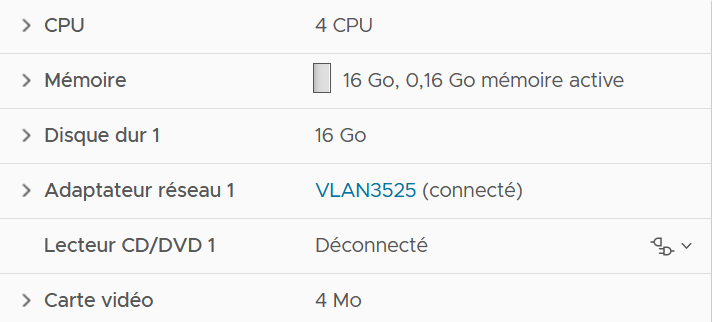
\includegraphics{images/CaracVM.png}
			\caption{Server in the PaaS}
			\label{server}
		\end{center}
	\end{figure}
	
	\section{Data Collection}
	
	In order to collect the data, we wrote the code for a server that makes requests to various APIs we want to access, which have interesting information.
	
	The different APIs are as follows:
	
	\begin{itemize}[noitemsep]
		\item STIB Open Data Portal : For all real-time data and static GTFS data.
		\item TLC API : For data concerning traffic lights.
		\item M3 API : For counting data provided by ANPR cameras.
	\end{itemize} 
	
	\textbf{Additional details to be added later, which I haven't thought of yet.} 
	
	
	\section{STIB}
	
	\subsection{Open Data Portal (ODP)}
	
	
	There are different sources of data provided to us through the STIB open data portal. As we can see in the figure \ref{STIB ODP}, it is possible to link a large portion of the data to which we have access in order to cover a maximum number of use cases that may interest us.
	
	
	\begin{figure}
		\centering
		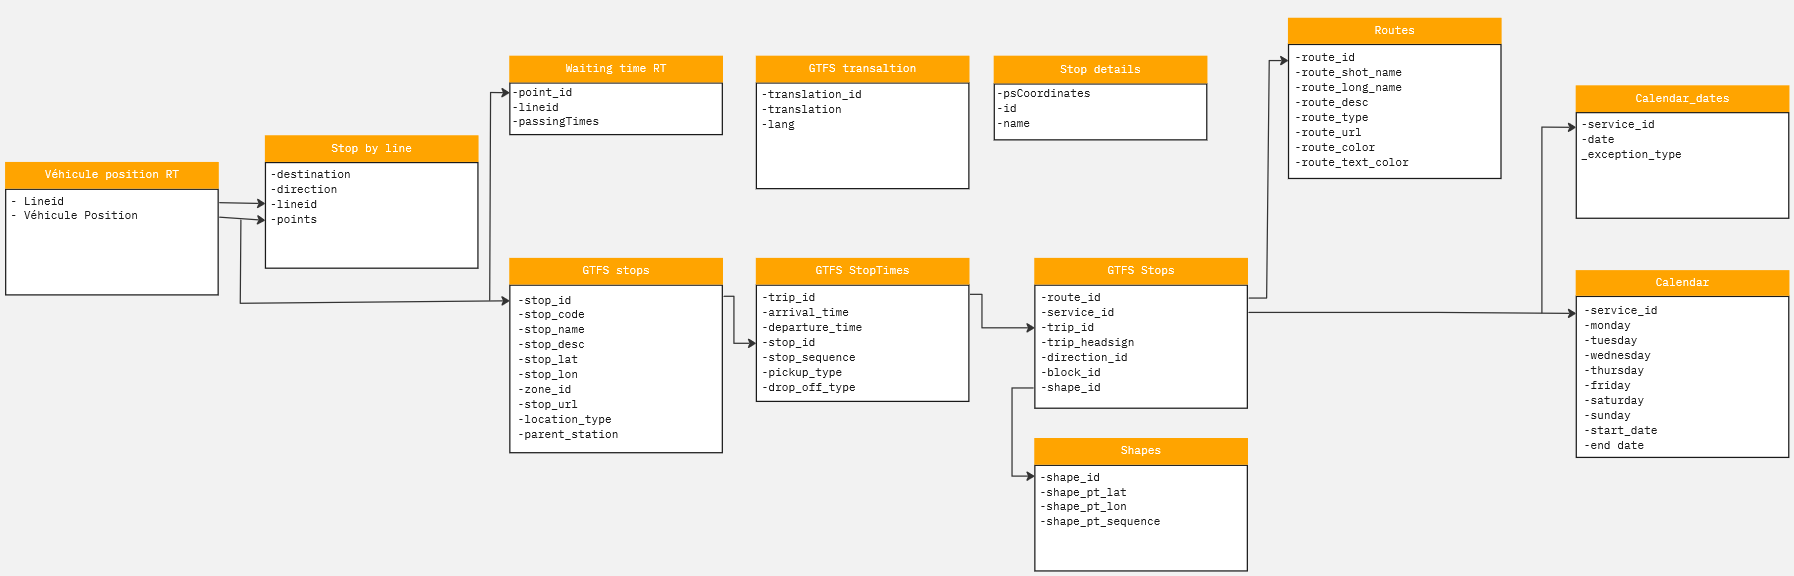
\includegraphics[angle=90,origin=c,scale=0.7]{images/tables GTFS.png}
		\caption{Data available on the open portal of the STIB}
		\label{STIB ODP}
	\end{figure}
	
	We will review the various tables to determine what is at our disposal and what we will use.
	
	\subsubsection{Vehicle Position RT}
	
	This part of the API provides us with significant information for the study of mobility, namely the last known position of all circulating STIB vehicles at any given moment. 
	
	The data is provided in JSON format and follows a schema as follows:
	
	\begin{figure}
		\centering
		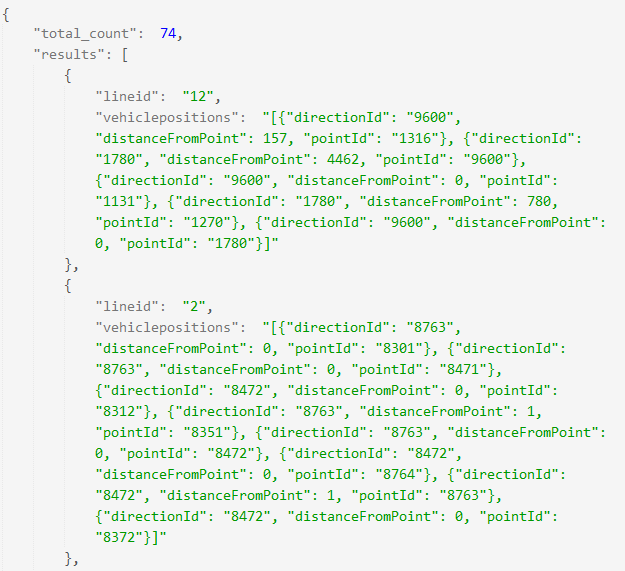
\includegraphics[width=\textwidth]{images/RTResponseJson}
		\caption{Vehicles position in RT}
		\label{RT_Position_content}
	\end{figure}
	
	
	The JSON file provides us with various pieces of information:
	
	\begin{center}
		\begin{itemize}[noitemsep]
			\item \textbf{total\_count} : The total number of lines with at least one vehicle in circulation.
			\item \textbf{results} : The set of results for each STIB line.
		\end{itemize}
	\end{center}
	
	
	For each STIB line, we have various pieces of information:
	
	\begin{center}
		\begin{itemize}[noitemsep]
			\item \textbf{lineid} : the number of the line
			\item \textbf{vehiclepositions} : The set of positions for each vehicle on the line.
		\end{itemize}
	\end{center}
	
	As we can see in the image, the data is separated by line. For each line, we have three pieces of information for each vehicle that is moving on the line at the moment the query was made.
	
	The information is as follows:
	
	
	\begin{itemize}[noitemsep]
		\item \textbf{directionId} : The ID of the terminus of the line towards which the vehicle is heading.
		\item \textbf{distanceFromPoint} : This is the distance in meters that the bus has traveled since the last stop it passed.
		\item \textbf{pointID} : This is the ID of the last stop that the vehicle passed.
	\end{itemize}
	
	\subsubsection{Stop by line}
	
	This table allows us to know, for each line, the stops in the order in which they are taken by the various vehicles of the STIB.
	
	\begin{figure}
		\centering
		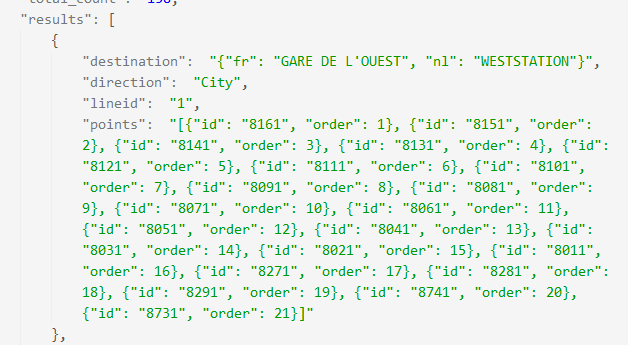
\includegraphics[width=\textwidth]{images/stops by line}
		\caption{Stops by line request result}
		\label{stops_by_line}
	\end{figure}
	
	As can be seen in Figure \ref{stops_by_line}, we have different data fields for each line: 
	
	\begin{itemize}[noitemsep]
		\item \textbf{destination} : the terminus of the line.
		\item \textbf{direction} : where the line ends.
		\item \textbf{points} : A list of data pairs with the stop number in order and its ID.
	\end{itemize}
	
	\subsubsection{Waiting times RT}
	
	This dataset allows us to know how soon the next two vehicles of the line will arrive for each stop on the STIB network.
	
	\begin{figure}
		\centering
		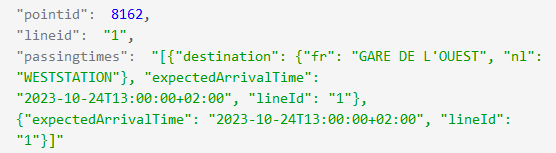
\includegraphics[width=\textwidth]{images/waiting_times}
		\caption{Waiting times RT request  result}
		\label{waiting_times}
	\end{figure}
	
	As we can see in Figure \ref{waiting_times}, the different data fields obtained are as follows:
	
	\begin{itemize}[noitemsep]
		\item \textbf{destination} : The stop at which the vehicles will arrive.
		\item \textbf{lineid} : The id of the line
		\item \textbf{passingTimes} : The estimated arrival time for the next two vehicles at the stop specified in the "destination" field.
	\end{itemize}	
	
	\subsubsection{GTFS Dataset}
	
	GTFS, which stands for General Transit Feed Specification, is a standardized format used to describe public transportation systems, making it easy for developers, transit agencies, and third-party applications to access and display information about public transit services. GTFS primarily consists of a set of plain text files containing structured data that provides a clear and comprehensive representation of a public transportation system.
	
	Here are the different data that follow the standard of GTFS that STIB provide through the open data portal.
	
	\begin{itemize}[noitemsep]
		\item \textbf{agency.txt} : This file contains details about the transit agency, including its name, URL, and contact information. It establishes the agency's identity within the dataset. 
		\item \textbf{stops.txt} : Lists all the stops within the transportation network, including their unique IDs, names, coordinates (latitude and longitude), and stop codes.
		\item \textbf{routes.txt} : Describes the various routes operated by the agency. It includes route names, IDs, and other attributes such as route type (bus, subway, tram, etc.).
		\item \textbf{trips} : Defines the specific trips or journeys that vehicles make on each route. It associates a trip with a route, service, and other information.
		\item \textbf{stop\_times.txt} : Contains detailed scheduling information for each trip, listing the times when vehicles arrive and depart from each stop. It includes arrival and departure times, stop IDs, and sequence information.
		\item \textbf{calendar.txt} : Provides a calendar of service, specifying the days of the week when services are active and date ranges for service exceptions like holidays.
		\item \textbf{calendar\_dates.txt} : Lists dates that have exceptions to the regular service schedule, indicating dates when a specific service is added or excluded.
		\item \textbf{shapes.txt} : Contains the spatial data representing the geographic paths of routes, often used for mapping and visualization purposes.
	\end{itemize}
	
	\subsubsection{Stop details}
	
	This data set is almost the same than the data provides in the "\textbf{stop.txt}" file of the GTFS dataset. The difference is that there is less details, the only that  availlable for each  stop are: 
	
	
	
	
	\begin{itemize}[noitemsep]
		\item \textbf{gpscoordinates} : the coordinate that we store in the WKB format after creating a PostGIS point with the longitude and latitude provided in the data.
		\item \textbf{stopid} : The id of the stop as in the stops data of the GTFS dataset
		\item \textbf{name} : The french translation of the stop's name
	\end{itemize}
	
	\begin{center}
		\begin{figure}
			\centering
			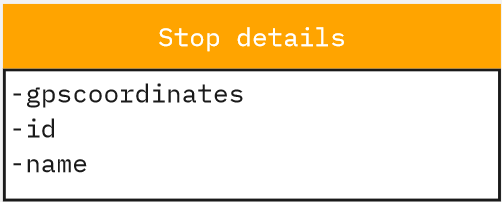
\includegraphics{images/stopDetailsTable.png}
			\caption{Stop details table}
			\label{stopDetailsTable}
		\end{figure}
	\end{center}
	
	The reason of the usage of both the stop details table provided by the STIB ans the stops table from the GTFS data set will be given and explained later. 
	
	\subsection{Storage}
	
	
	For STIB, real-time data is updated every 20 seconds, and considering that we take the values available at each update, we would need storage space equivalent to that listed in the table \ref{datasetsize}.
	
	
	\begin{table}
		\centering
		\begin{tabular}{|p{0.1\textheight}|c|c|c|c|c|c|}
			\hline
			Data & 20 seconds & 1 minute & 1 hour & 1 day & 1 month & 1 year \\
			\hline
			Positions RT & 37-60 Ko &  111-180 Ko & 6.7-10.8 Mo & 160.8-259.2 Mo & 4 Go-7.8 Go & 48-93.6 Go\\
			\hline
			Waiting Times RT & 1.15 Mo & 3.46 Mo & 208 Mo & 4.75 Go & 142.7 Go & 1.67 To \\
			\hline
			
		\end{tabular}
		\caption{Growth of dataset size gradually over time}
		\label{datasetsize}
	\end{table}
	
	
	
	We can already observe with the table above a difference in size between the two data sources. This is easily explained by the fact that on one hand, we have information concerning all vehicles in circulation, while on the other hand, it involves all stops in the STIB network, resulting in a significant difference in the size of the two datasets.
	
	
	\subsection{Process}
	
	The process of data collection and processing is visible in the image \ref{stib_data_process}, and the different steps will be explained in the following sections.
	
	
	\begin{center}
		\begin{figure}
			\centering
			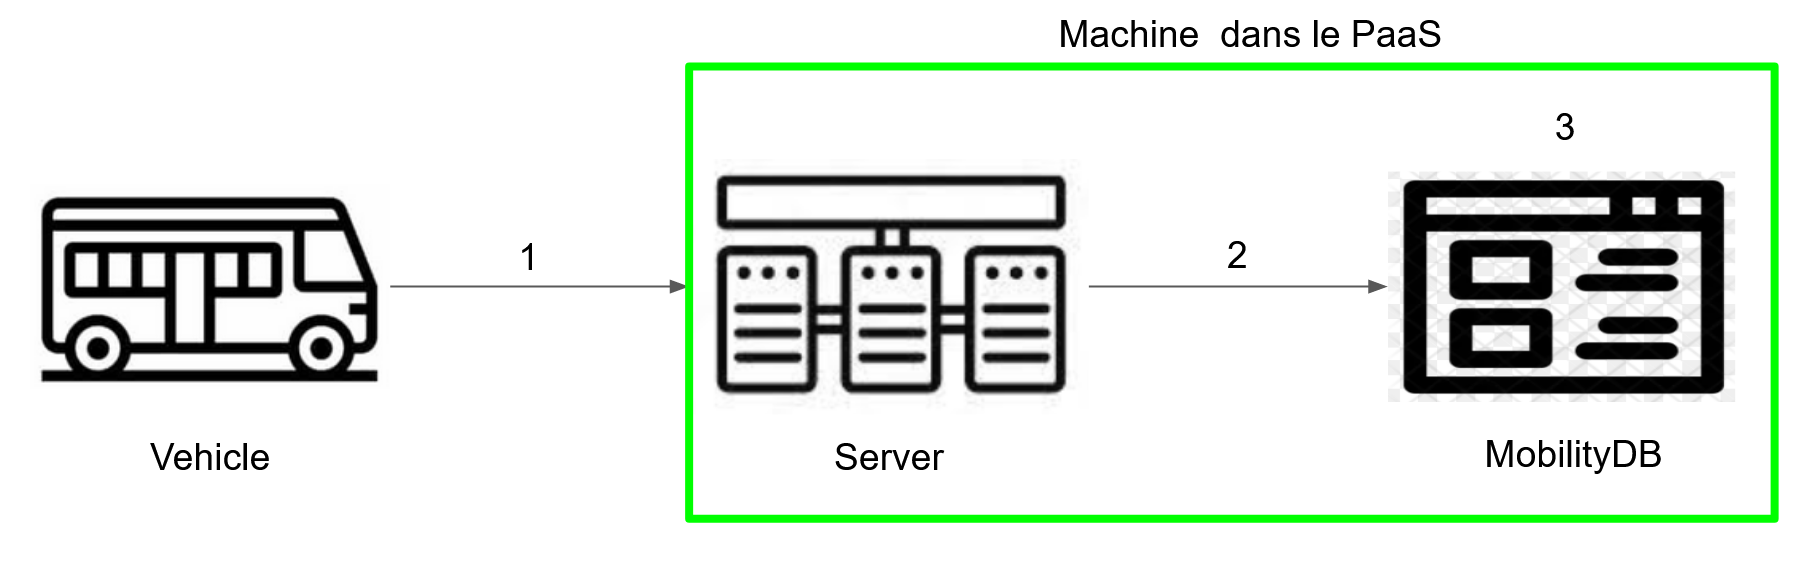
\includegraphics[width=0.9\textwidth]{images/stib_data_process.png}
			\caption{Process of STIB data}
			\label{stib_data_process}
		\end{figure}
	\end{center}
	
	There are three steps :
	
	\begin{itemize}[noitemsep]
		\item \textbf{1} : This simply involves the sending of data by the vehicles and their retrieval via the STIB \acrshort{odp}.
		
		\item \textbf{2} : Data collection via an API request that then executes queries on the database.
		
		\item \textbf{3} : Update of the mobilityDB trips
	\end{itemize}
	
	
	As indicated in Figure \ref{stib_data_process}, both the server and the database are installed on a machine on the PaaS network provided by BM. The characteristics of the latter are detailed in Figure \ref{server}.
	
	
	\subsection{Real-Time Position and Reverse Engineering}
	\label{sec:RT&reverseEngineering}
	
	One of the data sources that interests us the most is the one that allows us to know the real-time position of STIB vehicles. These are updated once every 20 seconds, in accordance with the information provided by the provider.
	
	The data is provided as shown in Figure \ref{RT_Position_content}.
	
	
	
	So, a question arises: What does the \textbf{distanceFromPoint} data really represent? Two possibilities are available to us:
	
	\begin{center}
		\begin{itemize}[noitemsep]
			\item \textbf{Rayon de cercle} : This is the as-the-crow-flies distance at which the vehicle is located relative to the last stop it was at.
			\item \textbf{Trajectoire} : This is the number of meters traveled by the vehicle following exactly the trajectory defined in the GTFS dataset shapefiles of the STIB.
		\end{itemize}
	\end{center}
	
	In the first case, we could obtain quite interesting information, but it would have lower precision since we cannot locate the vehicle accurately.
	
	In the second case, we would have much more precision as we can implement a system allowing us to calculate the almost exact position of the vehicle in terms of x and y coordinates through interpolation.
	
	The method used to determine which solution was more plausible is as follows.
	
	Firstly, data collection was necessary. Therefore, we ran a data catcher for several hours to obtain a sample of data as varied as possible.
	
	Now we needed to find a section of the route taken by a STIB vehicle where the trajectory is as non-linear as possible for the test to be as reliable as possible. The chosen section is shown in Figure \ref{Trancon17}, which is the route between the stops \textbf{Les 3 Tilleuls} and \textbf{Miraval}.
	
	\begin{center}
		\begin{figure}
			\centering
			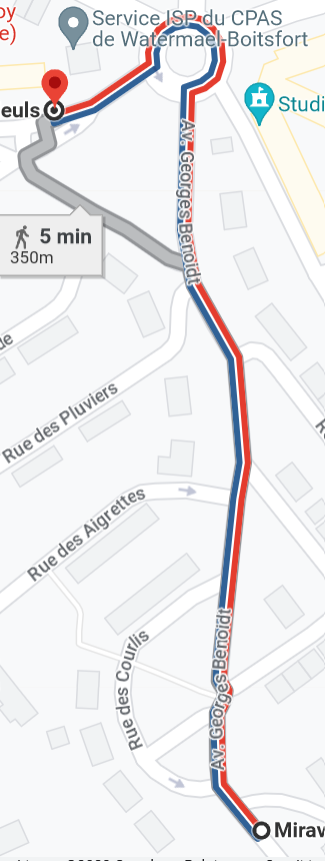
\includegraphics{images/trancon17.png}
			\caption{Trancon trajet bus 17 et 95}
			\label{Trancon17}
		\end{figure}
	\end{center}
	
	By sorting the captured data, we could make a selection to view only the data of the buses on the section of interest. All of this can be done using Excel with some fairly simple formulas. The result obtained is visible in Figure \ref{excelPositionRT}.
	
	\begin{center}
		\begin{figure}
			\centering
			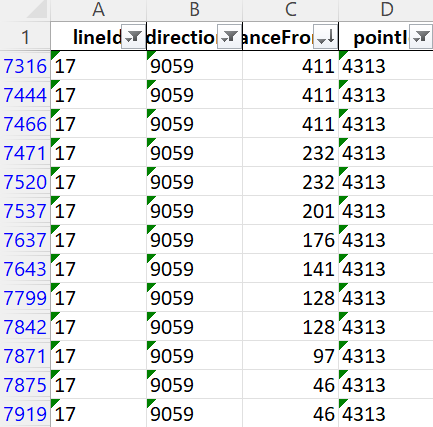
\includegraphics{images/excel position rt.png}
			\caption{Data recolted}
			\label{excelPositionRT}
		\end{figure}
	\end{center}
	
	\vspace{-2cm}	
	Let's take the largest recorded value and compare it to the distance between the two stops. The distance between the two stops can be read on Figure \ref{trancon17distance}. We end up with a difference of two meters between the recorded data and the value that can be found using Google Maps.
	
	\begin{center}
		\begin{figure}
			\centering
			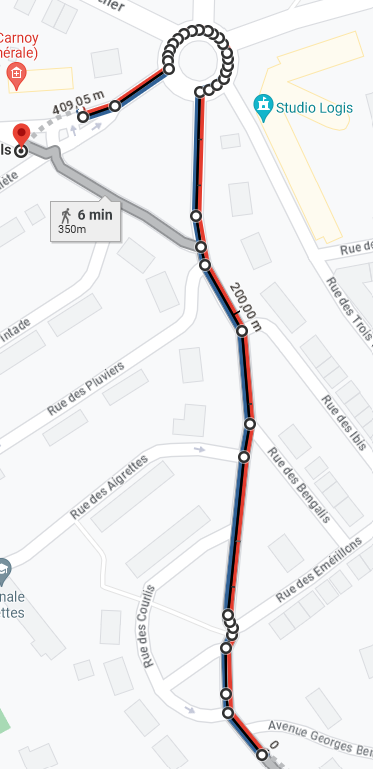
\includegraphics{images/tranconsBus17-3Till-Miraval.png}
			\caption{Trancon trajet bus 17 et 95}
			\label{trancon17distance}
		\end{figure}
	\end{center}
	
	\vspace{-2cm}
	
	Now that we know exactly what the \textbf{distanceFromPoint} data represents, namely the number of meters traveled on the predefined trajectory of the vehicle, we can apply the proposal made earlier. Namely, an interpolation that will allow us to obtain the exact coordinates of the vehicle for a more interesting analysis of its behavior using the functionalities available in MobilityDB.
	
	\subsection{Interpolation and Trip Construction}
	
	In this section, we will discuss the method used to construct MobilityDB trips based on the data made available to us on the STIB \acrshort{odp}.
	
	\subsubsection{Interpolation}
	
	The data received via the STI\acrshort{odp} from the production of real-time vehicle positions is not sufficient to allow us to construct a MobilityDB trip. Therefore, we need a way to derive real coordinates from the three fields we receive in the result of our API query.
	
	We start with three pieces of information:
	
	\begin{itemize}[noitemsep]
		\item \textbf{directionId} : The id of the terminus
		\item \textbf{distanceFromPoint} : Distance traveled since the last point following the predefined trajectory of the vehicle's route.
		\item \textbf{pointId} : The ID of the stop from which the distance was measured.
	\end{itemize}  
	
	
	As we can see in Figure \ref{conversionProblem}, it is challenging to locate the vehicle on the predefined trajectory with just a distance. This is where the interpolation calculation comes in, which will allow us to obtain GPS coordinates from RT data. Before performing the interpolation calculation, it is necessary to first check whether the vehicle is in deviation or not. In the event that it is, we cannot carry out the interpolation due to a lack of information. The process is illustrated in Figure \ref{diagramDeviation}.
	
	\begin{center}
		\begin{figure}
			\centering
			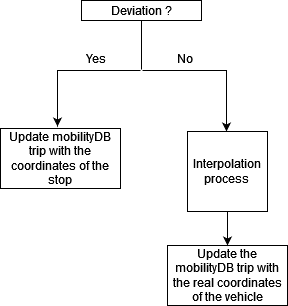
\includegraphics[width=0.4\textwidth]{images/diagram deviation.png}
			\caption{Diagram montrant le choix en cas de déviation.}
			\label{diagramDeviation}
		\end{figure}
	\end{center}
	
	\begin{center}
		\begin{figure}
			\centering
			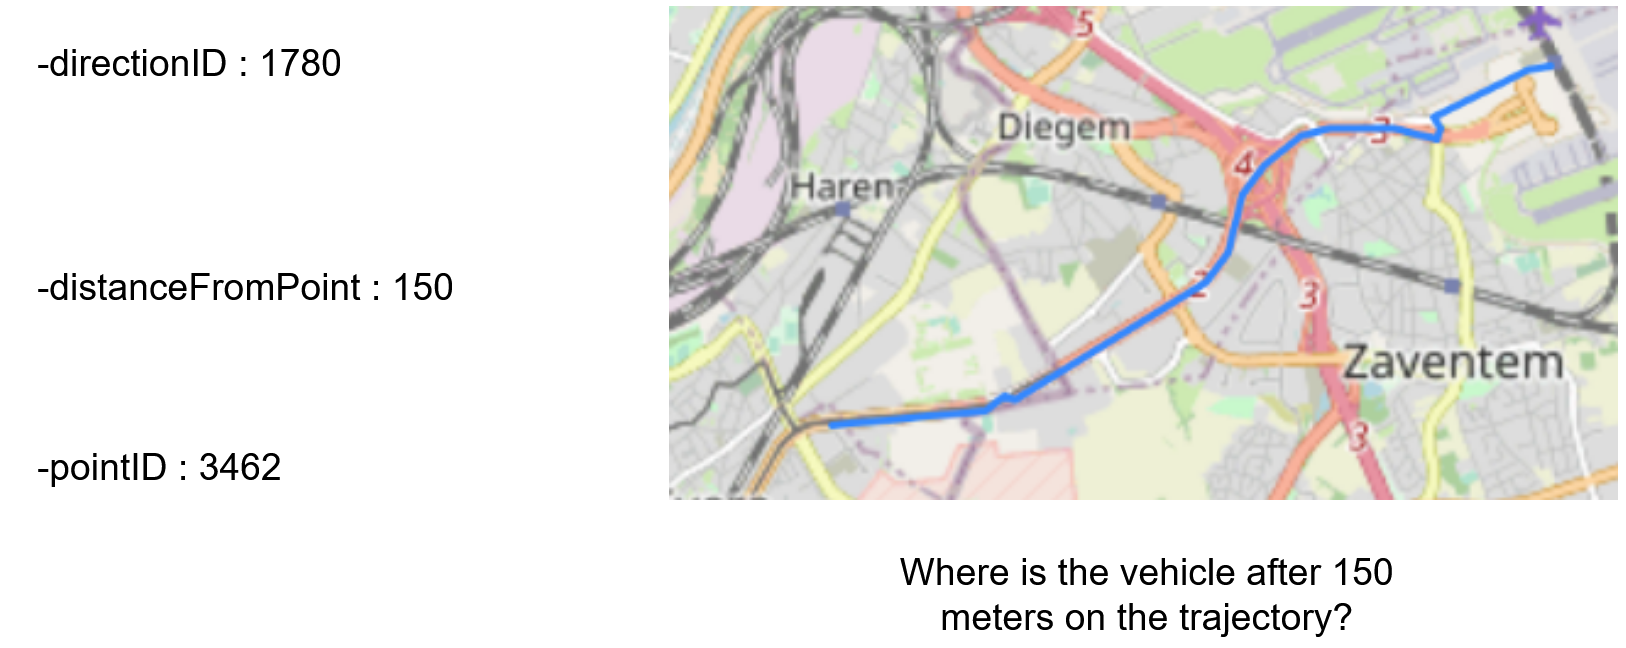
\includegraphics[width=0.9\textwidth]{images/conversionProblem.png}
			\caption{Description of the problem when receiving the data}
			\label{conversionProblem}
		\end{figure}
	\end{center}
	
	
	\vspace{-3cm}
	
	To do this, we need to make certain queries to obtain everything that is necessary.
	
	The first step is to isolate the part of the trajectory between the last visited stop and the end of the line. Therefore we need to find the coordinates of the last visited stop. To do this, we use the query \ref{rightIdCoord}.
	
	\begin{lstlisting}[language=SQL,
		caption={Query  to find the right id for the terminus and the coordinates for the stop},
		label={rightIdCoord},
		basicstyle={\small\ttfamily},
		belowskip=3mm,
		breakatwhitespace=true,
		breaklines=true,
		classoffset=0,
		columns=flexible,
		commentstyle=\color{dkgreen},
		framexleftmargin=0.25em,
		frameshape={}{yy}{}{}, %To remove to vertical lines on left, set `frameshape={}{}{}{}`
		keywordstyle=\color{blue},
		numbers=left, %If you want line numbers, set `numbers=left`
		numberstyle=\tiny\color{gray},
		showstringspaces=false,
		stringstyle=\color{mauve},
		tabsize=3,
		xleftmargin =1em]
		
		--get the real id terminus
		SELECT stopid as stop  from  stopdetails where stopid LIKE '%' || directionID || '%'
		--Get coordinate of the stop 
		SELECT ST_SetSRID(ST_MakePoint(p1.stop_lon,p1.stop_lat),4326) as point1
		FROM stops as p1
		WHERE p1.stop_id  LIKE '%' || pointID || '%'  --Replace by pointID
		
	\end{lstlisting}
	
	
	Once the terminus and the point are found, we can select the shape associated with the route using the ID of the terminus and the fraction of the route using the point of the last visited stop. This selection of the fraction is done using queries \ref{startsubtraj} and \ref{subfracQuery}.
	
	
	\begin{lstlisting}[language=SQL,
		caption={Query to  find the start of the subtrajectory},
		label={startsubtraj},
		basicstyle={\small\ttfamily},
		belowskip=3mm,
		breakatwhitespace=true,
		breaklines=true,
		classoffset=0,
		columns=flexible,
		commentstyle=\color{dkgreen},
		framexleftmargin=0.25em,
		frameshape={}{yy}{}{}, %To remove to vertical lines on left, set `frameshape={}{}{}{}`
		keywordstyle=\color{blue},
		numbers=left, %If you want line numbers, set `numbers=left`
		numberstyle=\tiny\color{gray},
		showstringspaces=false,
		stringstyle=\color{mauve},
		tabsize=3,
		xleftmargin =1em]
		SELECT
		ST_LineLocatePoint(trajectory.trajectory, point1) AS start_fraction
		FROM
		terminus_shapes AS trajectory 
		WHERE
		trajectory.route_short_name = lineID 
		AND trajectory.stopid = directionID
	\end{lstlisting}
	
	
	\begin{lstlisting}[language=SQL,
		caption={Query that select the subfraction of the trajectory},
		label={subfracQuery},
		basicstyle={\small\ttfamily},
		belowskip=3mm,
		breakatwhitespace=true,
		breaklines=true,
		classoffset=0,
		columns=flexible,
		commentstyle=\color{dkgreen},
		framexleftmargin=0.25em,
		frameshape={}{yy}{}{}, %To remove to vertical lines on left, set `frameshape={}{}{}{}`
		keywordstyle=\color{blue},
		numbers=left, %If you want line numbers, set `numbers=left`
		numberstyle=\tiny\color{gray},
		showstringspaces=false,
		stringstyle=\color{mauve},
		tabsize=3,
		xleftmargin =1em]
		SELECT
		ST_SetSRID(ST_LineSubstring(trajectory.trajectory, strat_fraction,1),4326) AS sub_trajectory
		FROM
		terminus_shapes AS trajectory
		WHERE 
		trajectory.route_short_name = lineID AND trajectory.stopid = directionID
		limit 1
	\end{lstlisting}
	
	With these queries, we can isolate the section of the route that allows us to find the real coordinates of the vehicle through interpolation.
	
	Interpolation is done by executing the query \ref{interpolationQuery}.
	
	\begin{lstlisting}[language=SQL,
		caption={Query that calculate the interpolation},
		label={interpolationQuery},
		basicstyle={\small\ttfamily},
		belowskip=3mm,
		breakatwhitespace=true,
		breaklines=true,
		classoffset=0,
		columns=flexible,
		commentstyle=\color{dkgreen},
		framexleftmargin=0.25em,
		frameshape={}{yy}{}{}, %To remove to vertical lines on left, set `frameshape={}{}{}{}`
		keywordstyle=\color{blue},
		numbers=left, %If you want line numbers, set `numbers=left`
		numberstyle=\tiny\color{gray},
		showstringspaces=false,
		stringstyle=\color{mauve},
		tabsize=3,
		xleftmargin =1em]
		SELECT ST_LineInterpolatePoint(st.sub_trajectory, distanceFromPoint/ST_Length(st.sub_trajectory::geography))
		FROM sub_trajectory  as st
	\end{lstlisting}
	
	
	Once all these queries are executed, we have real coordinates that allow us to construct our MobilityDB trips.
	
	It is interesting to see now how trips are updated in the database. Regarding the insertion of a new trip or the update of a trip that has already started, this is done using the function\ref{fonctionInsert}
	
	\begin{lstlisting}[language=SQL,
		caption={Function to update the table},
		label={fonctionInsert},
		basicstyle={\small\ttfamily},
		belowskip=3mm,
		breakatwhitespace=true,
		breaklines=true,
		classoffset=0,
		columns=flexible,
		commentstyle=\color{dkgreen},
		framexleftmargin=0.25em,
		frameshape={}{yy}{}{}, %To remove to vertical lines on left, set `frameshape={}{}{}{}`
		keywordstyle=\color{blue},
		numbers=left, %If you want line numbers, set `numbers=left`
		numberstyle=\tiny\color{gray},
		showstringspaces=false,
		stringstyle=\color{mauve},
		tabsize=3,
		xleftmargin =1em]
		CREATE OR REPLACE FUNCTION insert_or_update_stib_trip(
		p_day DATE, p_lineid TEXT, p_tripid TEXT, p_directionid TEXT,
		p_start_timestamp TIMESTAMPTZ, p_end_timestamp TIMESTAMPTZ,
		p_is_deviated BOOLEAN, p_current BOOLEAN, p_trip tgeompoint
		)
		RETURNS VOID AS $$
		BEGIN
		-- Check if there is an existing record with the same day, lineid, and tripid
		PERFORM 1
		FROM stib_trips
		WHERE day = p_day AND lineid = p_lineid AND tripid = p_tripid AND directionid = p_directionid AND current;
		
		IF FOUND THEN
		-- Update the existing record
		UPDATE stib_trips
		SET
		end_timestamp = p_end_timestamp,
		is_deviated = p_is_deviated,
		trip = update_trip(p_trip, stib_trips.trip)
		WHERE
		day = p_day AND lineid = p_lineid AND tripid = p_tripid AND directionid = p_directionid AND current;
		ELSE
		-- Set current to false for the previous record with the same day, lineid, and tripid
		UPDATE stib_trips
		SET
		current = false
		WHERE
		day = p_day AND lineid = p_lineid AND tripid = p_tripid;
		
		-- Insert a new record
		INSERT INTO stib_trips (day, lineid, tripid, directionid, start_timestamp, end_timestamp, is_deviated, current, trip)
		VALUES (p_day, p_lineid, p_tripid, p_directionid, p_start_timestamp, p_end_timestamp, p_is_deviated, p_current, p_trip);
		END IF;
		END;
		$$ LANGUAGE plpgsql;
		
		-- Define a function to calculate the updated value for trip  column
		CREATE OR REPLACE FUNCTION update_trip(new_tgeompoint tgeompoint, existing_tgeompoint tgeompoint)
		RETURNS tgeompoint AS $$
		DECLARE
		updated_tgeompoint tgeompoint;
		BEGIN
		SELECT appendInstant(existing_tgeompoint, new_tgeompoint) INTO updated_tgeompoint;
		RETURN updated_tgeompoint;
		END;
		$$ LANGUAGE plpgsql;
	\end{lstlisting}
	
	Here, the goal is to add a flag to each trip to indicate whether it is the current journey or not, using the \textbf{current} column in the table. To conclude the trip at the right moment, we use the \textbf{directionId} field of each vehicle received in the real-time data as the flag.
	
	To achieve this, we construct a map with the trip ID as the key and the terminus towards which the vehicle is heading as the value. In this way, when we receive real-time data and observe a change in the directionId of a vehicle, the flag that designates the current route is reversed, and a new line is added and marked as the one to be updated later.
	
	
	The trips are stored, as we can see in Figure \ref{table_trips}. 
	
	The reason why the trips have been stored in this way is that it allows for a better analysis in case of issues on the network. Isolating each round trip between the two terminus of a line makes it easy to identify which trip it is by using the vehicle's start and end timestamps.
	
	
	In the table, we find the following attributes: 
	
	\begin{itemize}[noitemsep]
		\item \textbf{day} : The day on which the trip was recorded.
		\item \textbf{lineid} : The id of the line.
		\item \textbf{tripid} : This is the vehicle ID, simply the concatenation of the line ID with the vehicle number in the real-time data received.
		\item \textbf{directionid} :The ID of the terminus towards which the vehicle is heading.
		\item \textbf{start\_timestamp} : The timestamp from which the trip started to be recorded.
		\item \textbf{end\_timestamp} : The timestamp indicating the end of the trip.
		\item \textbf{is\_deviated} : A boolean indicating whether there is a deviation on the line during the recording period of the trip.
		\item \textbf{current} : The boolean that serves as a flag to determine if the trip to be updated is the correct one.
		\item \textbf{Trip} : The tgeompoint used for the analysis of vehicle movement data.
	\end{itemize}
	
	
	
	\begin{center}
		\begin{figure}
			\centering
			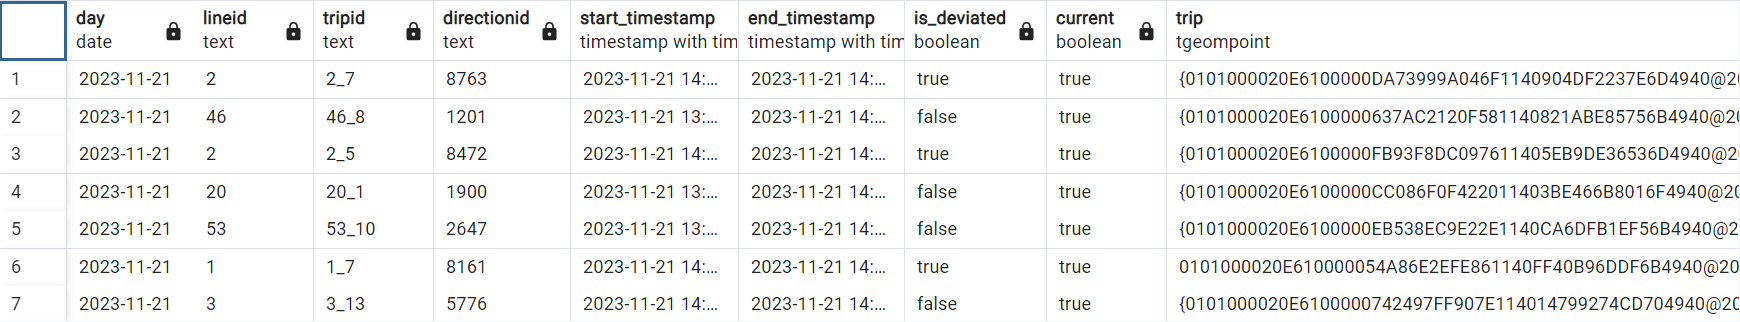
\includegraphics[width=0.9\textwidth]{images/stib_table_trips.png}
			\caption{Tables containing mobilityDB trips}
			\label{table_trips}
		\end{figure}
	\end{center}
	
	
	
	\subsection{Encountered Problems}
	\label{sec:EncouteredProblemsTIB}
	
	We encountered various problems during the analysis of \acrshort{stib} data, which means that the obtained result is not entirely real or that we cannot achieve a certain degree of precision in our data.
	
	The first problem encountered, which poses an issue in the construction of MobilityDB trips, is the absence of IDs to distinguish the different vehicles circulating on the \acrshort{stib} network.
	
	The second problem is the absence of certain stops in the \acrshort{stib} network's stop dataset. This is problematic for interpolation calculations because the inability to find a stop prevents us from selecting the correct shape for interpolation.
	
	The last problem is the lack of compatibility between real-time and static data provided in the GTFS dataset. This difference means that some deviations are impossible to reconstruct in MobilityDB trips because the corresponding shapes are not available.
	
	\section{TLC API}
	
	In this section we will discuss about the  data that TLC provides to BM in order to visualize the state of traffic lights at any moment anywhere in Brussels.
	
	In the development of analytical tools utilized within this research, a critical data acquisition process is implemented, initiated by an application program interface (API) call to the designated traffic portal. This initial request, as designed by a contributor to the project named Sven, is required to specify the 'CLE'—a concise identifier utilized within Scala programming—and a commencement timestamp. The provision for an optional termination timestamp is also incorporated to delineate the temporal scope of the data retrieval (Sven, 2023) as shown in Figure \ref{TLCRequest} and Table \ref{table_param_TLC}.
	
	\begin{center}
		\begin{figure}
			\centering
			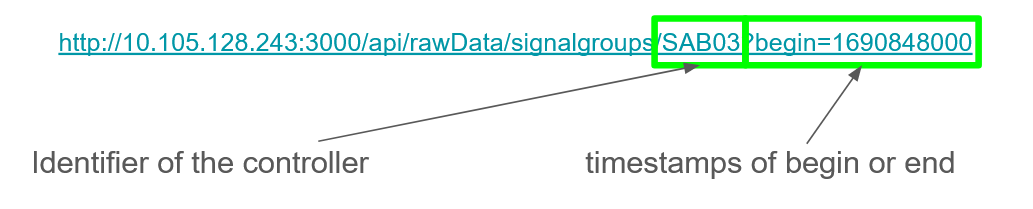
\includegraphics[width=0.9\textwidth]{images/TLCRequest.png}
			\caption{TLC request example}
			\label{TLCRequest}
		\end{figure}
	\end{center}
	
	\begin{table}
		\centering
		\begin{tabular}{|p{0.1\textheight}|c|c|c|c|}
			\hline
			Name & Type & Default & Required  \\
			\hline
			begin & Unix Timestamp & Now - 1 hour & False\\
			\hline
			end & Unix Timestamp & Now & False \\
			\hline
			
		\end{tabular}
		\caption{Parameter that can be added to the API request}
		\label{table_param_TLC}
	\end{table}
	
	\vspace{-2cm}
	Subsequent to the initiation request, the traffic portal conducts a validation of both the 'CLE' and the temporal parameters. This step is preliminary to the procurement of comprehensive data from the suite of detectors and signal groups that correspond to the control point of interest, spanning the requested time frame. The culmination of this process is the generation of a data file, formatted in either JSON or XML as per the established agreement, which encapsulates the gathered data (Sven, 2023).
	
	It is pertinent to note that the data originates from the Scala database (IG), with an imposed latency of five minutes on the most recent records, thereby excluding data within this quintuple-minute timeframe from the retrieval process.
	
	The operational remit of the traffic portal extends to the translation of the API call into the OCIT-C protocol. This translation is accompanied by a series of verifications pertaining to the authenticity of the request and the availability of the data. The final phase involves the portal's conversion of the OCIT-C data response, as received from the IG, back into a user-friendly JSON or XML format \footnote{This informations are in a word file that Sven from BM shared with  us}. All this process can be visualized in the Figure \ref{TLCProcess}.
	
	\begin{center}
		\begin{figure}
			\centering
			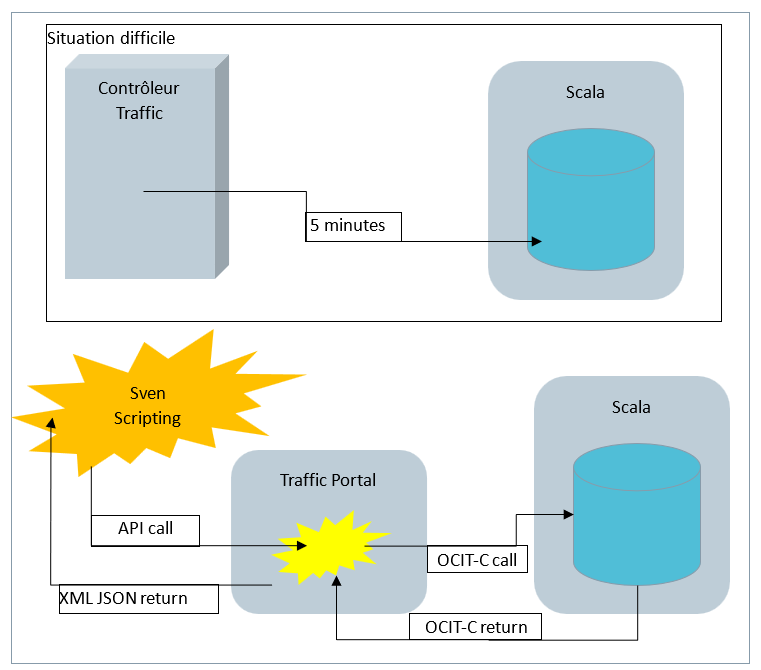
\includegraphics[width=0.9\textwidth]{images/TLCProcess.png}
			\caption{Entire process between requesting data and receiving response.}
			\label{TLCProcess}
		\end{figure}
	\end{center}
	
	\vspace{-2cm}
	Once all the process is completed,we receive the response in the format of a JSON file. The metadata of the responsone is give in the Table \ref{tab:data_structure} and  an image of the JSON response is showed in  Figure \ref{ResponseJSONTLC}.
	\vspace{-2cm}
	\begin{table}[ht]
		\centering
		\begin{tabular}{|l|l|p{5cm}|l|}
			\hline
			\textbf{Field} & \textbf{Type} & \textbf{Description} & \textbf{Example} \\ \hline
			tstore & DateTime & Moment the data was stored & 2021-04-01T18:43:31.648+02:00 \\ \hline
			identifier/ident & String & Central intersection No & J1\_12\_40 \\ \hline
			rawData ID & String & Name of the signal group & "Id": "J8" \\ \hline
			Timestamp & DateTime & Holds the measurement timestamp & 2021-04-02T07:38:59.270+02:00 \\ \hline
			intervalLength & Int & Time unit in milliseconds & 1 \\ \hline
			Data Value & Int & \begin{minipage}[t]{5cm}\raggedright
				Identifies the state of the detector:
				\begin{itemize}[noitemsep]
					\item 0: black
					\item 3: red
					\item 12: orange
					\item 15: Red-Orange
					\item 32: green blinking
					\item 48: green
				\end{itemize}
			\end{minipage} & \begin{tabular}[c]{@{}l@{}}Value: "3"\\ Value: "48"\end{tabular} \\ \hline
			Data Offset & Int & milliseconds after the timeline timestamp where the detector state changed & “offset”: 33230 \\ \hline
		\end{tabular}
		\caption{Data Structure Description}
		\label{tab:data_structure}
	\end{table}
	
	\begin{center}
		\begin{figure}
			\centering
			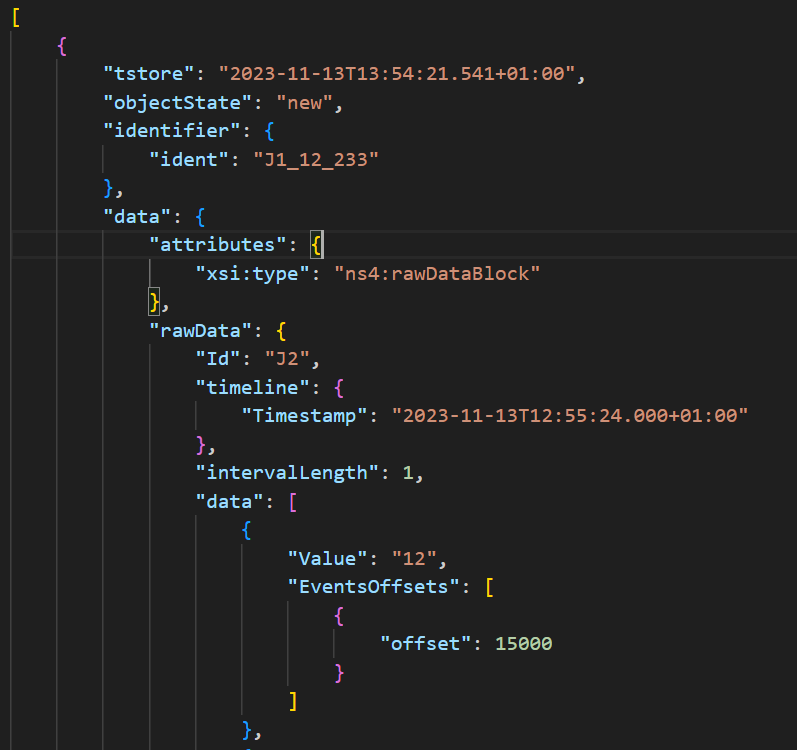
\includegraphics[width=0.9\textwidth]{images/ResponseJSONTLC.png}
			\caption{JSON file received as response from TLC API request}
			\label{ResponseJSONTLC}
		\end{figure}
	\end{center}
	
	
	For the moment any work has been done with this data and every thing will be explained in Section \ref{sec:futurWorkTLC} from why we cannot work on it for the moment and what could be done with this data.
	
	\section{M³ API}
	\label{sec:dataM3}
	
	In this section we will take a look to de that that is provided by the ANPR cameras that we talked about Section \ref{sec:M3}. First of all let's take a look at the process to retrieve the data as it is showed in Figure \ref{AnprDataTransfer}, we can see that kafka is  used to stream the data and this is explained by all the reasons given in Section \ref{sec:kafka}. 
	
	\begin{center}
		\begin{figure}
			\centering
			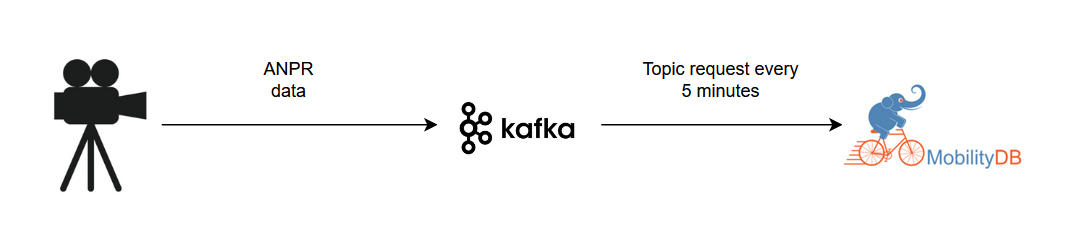
\includegraphics[width=0.9\textwidth]{images/AnprDataTransfer.png}
			\caption{Transfer process of ANPR data}
			\label{AnprDataTransfer}
		\end{figure}
	\end{center}
	
	There is two kind of data that are provided by M³, the  first categorie  is the counting of vehicle around a camera and the second one is the statistics about the average speeds of the vehicles between two cameras. Both file a represented by examples in Figures \ref{img:M3count} and \ref{img:M3stats}
	
	\begin{center}
		\begin{figure}
			\centering
			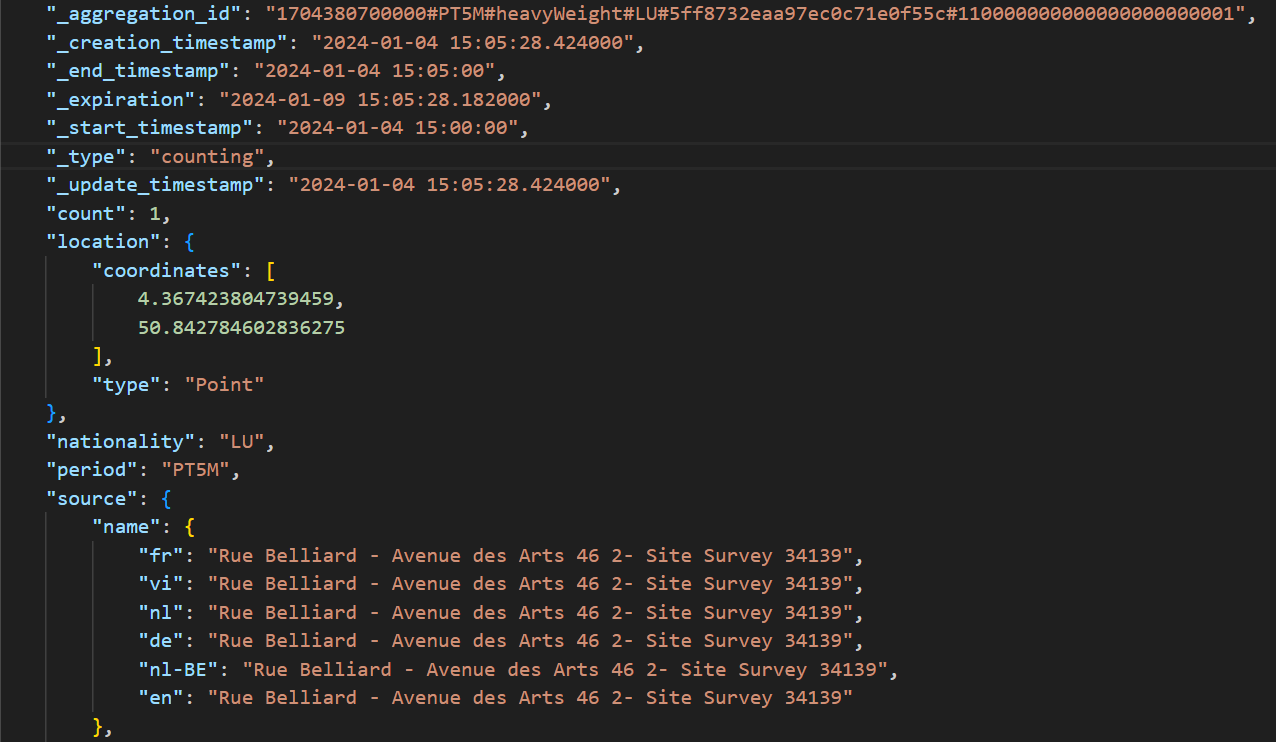
\includegraphics[width=0.9\textwidth]{images/M3count.png}
			\caption{Example of counting data}
			\label{img:M3count}
		\end{figure}
	\end{center}
	
	\begin{center}
		\begin{figure}
			\centering
			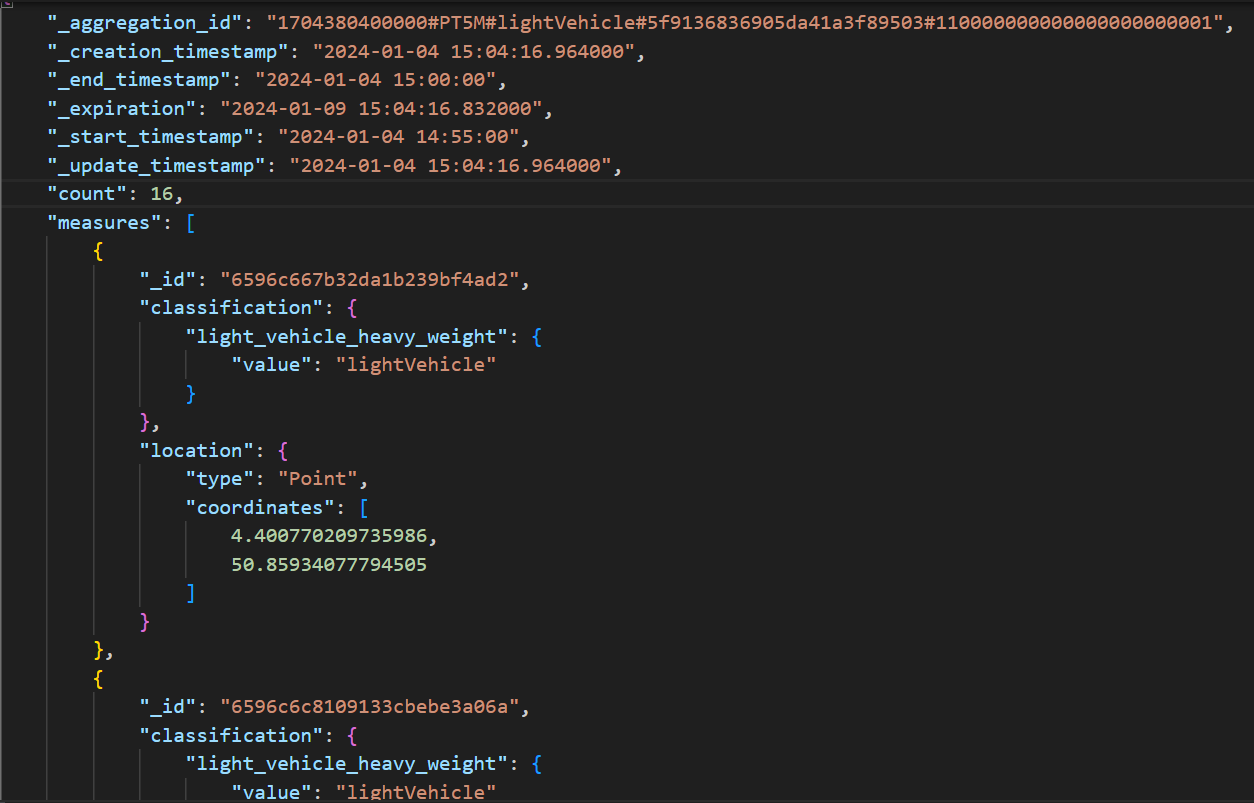
\includegraphics[width=0.9\textwidth]{images/M3stats.png}
			\caption{Example of speed statistic data}
			\label{img:M3stats}
		\end{figure}
	\end{center}
	
	
	
	\chapter{Added Values and Use Cases}
	
	In this chapter we will go through the results of all the implementations that have been done or have been analyzed in order to allow the futures persons that will continue this work to have a clear vision of what is expected from them. There is 5 majors path to follow : 
	
	\begin{itemize}[noitemsep]
		\item \textbf{Visualization tool}
		\item \textbf{\acrshort{stib} alarms}
		\item \textbf{\acrshort{stib} trip}
	\end{itemize}
	
	each of the works will be explained more in details in the respective section. We will discuss about the current state of the work, why it is complicated to go further and what could be added to improve the work.
	
	\section{\acrshort{stib} Trips}
	
	The main added value of  this work is the possibility to construct the trip for any vehicle of the STIB that is actually in service and is sharing  his data through Open Data Portal of the STIB. The features that will be described in next Sections are all based on the this one. In the scope of this work only two use cases have been developed but since we can construct MobilityDB trips we can use all the other functions that MobilityDB can propose.
	
	
	
	
	
	\section{Visualization Tool}
	
	In this section we will discuss about the visualization tool that has been implemented in order to visualize the data provided by the \acrshort{stib} through the \acrshort{odp}, and show the two visualisation tool that compose the main tool. The two part that compose it are  one base on the visualization of historical  data allowing to chose the moment that the user is interested to watch from the past and a tool to see the position of every vehicle in real-time. Both tools are written using the framework DeckGL and the technology of \acrlong{mvt} (\acrshort{mvt}) to allow better performances as explained in Section \ref{sec:MVT} and the usage of pg\_tileserv (that was presented in Section \ref{sec:pgTileServ}) as shown in figure \ref{processMVTVisu} .
	
	\begin{center}
		\begin{figure}
			\centering
			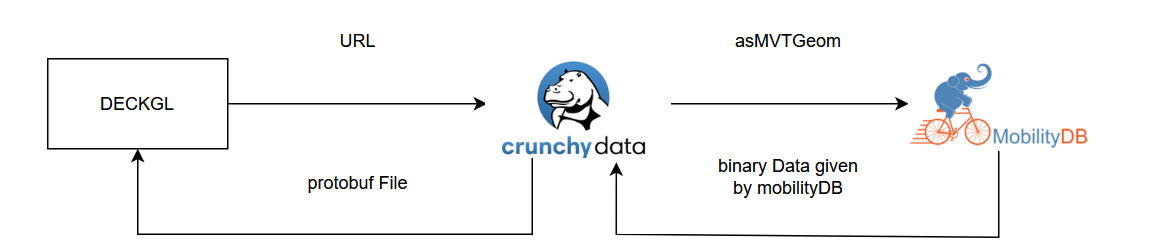
\includegraphics[width=0.9\textwidth]{images/processMVTVisu.png}
			\caption{Communication process to get the visualization}
			\label{processMVTVisu}
		\end{figure}
	\end{center}
	
	\subsection{Historical Data Visualization}
	
	The module under review in this segment is architected to streamline the process of examining vehicle dynamics within the STIB network historically. It confers upon users the capacity to designate specific temporal brackets for analysis, facilitating the observation of vehicle or line behaviors within those defined epochs, conditional upon data congruence for the period in question.
	
	Foremost, the module's functionalities bifurcate into two principal visualization modalities: the surveillance of individual vehicular movements and the aggregate tracing of line-wide transit patterns. Such a dichotomy permits an in-depth exploration of singular trajectories as well as comprehensive views of the network's flux. Nonetheless, it is crucial to acknowledge the granularity limitations of historical data. At times, these constraints precipitate the emergence of anomalous or implausible visual depictions, as exemplified in figure \ref{badDataHist}.
	
	\begin{center}
		\begin{figure}
			\centering
			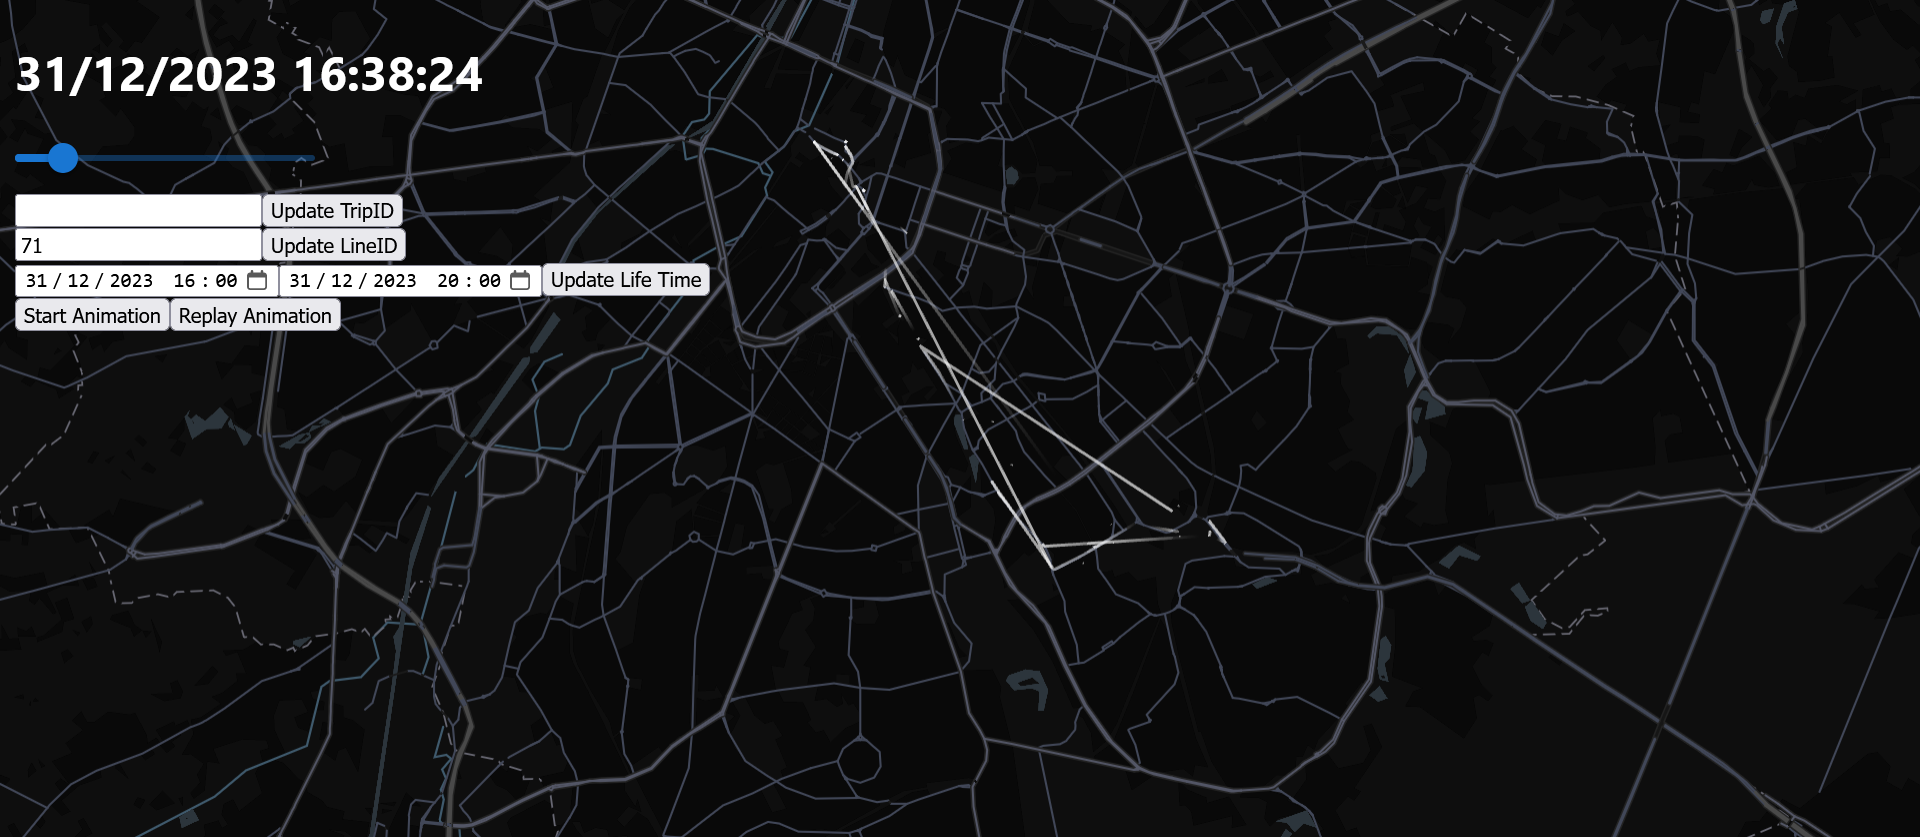
\includegraphics[width=0.9\textwidth]{images/BadDataHist.png}
			\caption{Displayed data make no sense}
			\label{badDataHist}
		\end{figure}
	\end{center}
	\vspace{-2cm}
	The visual apparatus, as depicted in Figure \ref{badDataHist}, is equipped with interactive mapping, temporal navigation, and animation controls. These instruments authorize the user to dynamically alter the visualization parameters, encompassing trip ID, line ID, and the data's lifecycle. While the visualization interface is meticulously engineered to yield an intuitive and educational exploration of the network's historical vehicle patterns, it must be conceded that data fidelity issues can sporadically induce atypical graphical representations. Despite these sporadic anomalies, the interface endeavors to furnish users with a coherent and insightful historical data visualization experience, consolidating its utility in the realm of urban transport network analysis.
	
	\begin{center}
		\begin{figure}
			\centering
			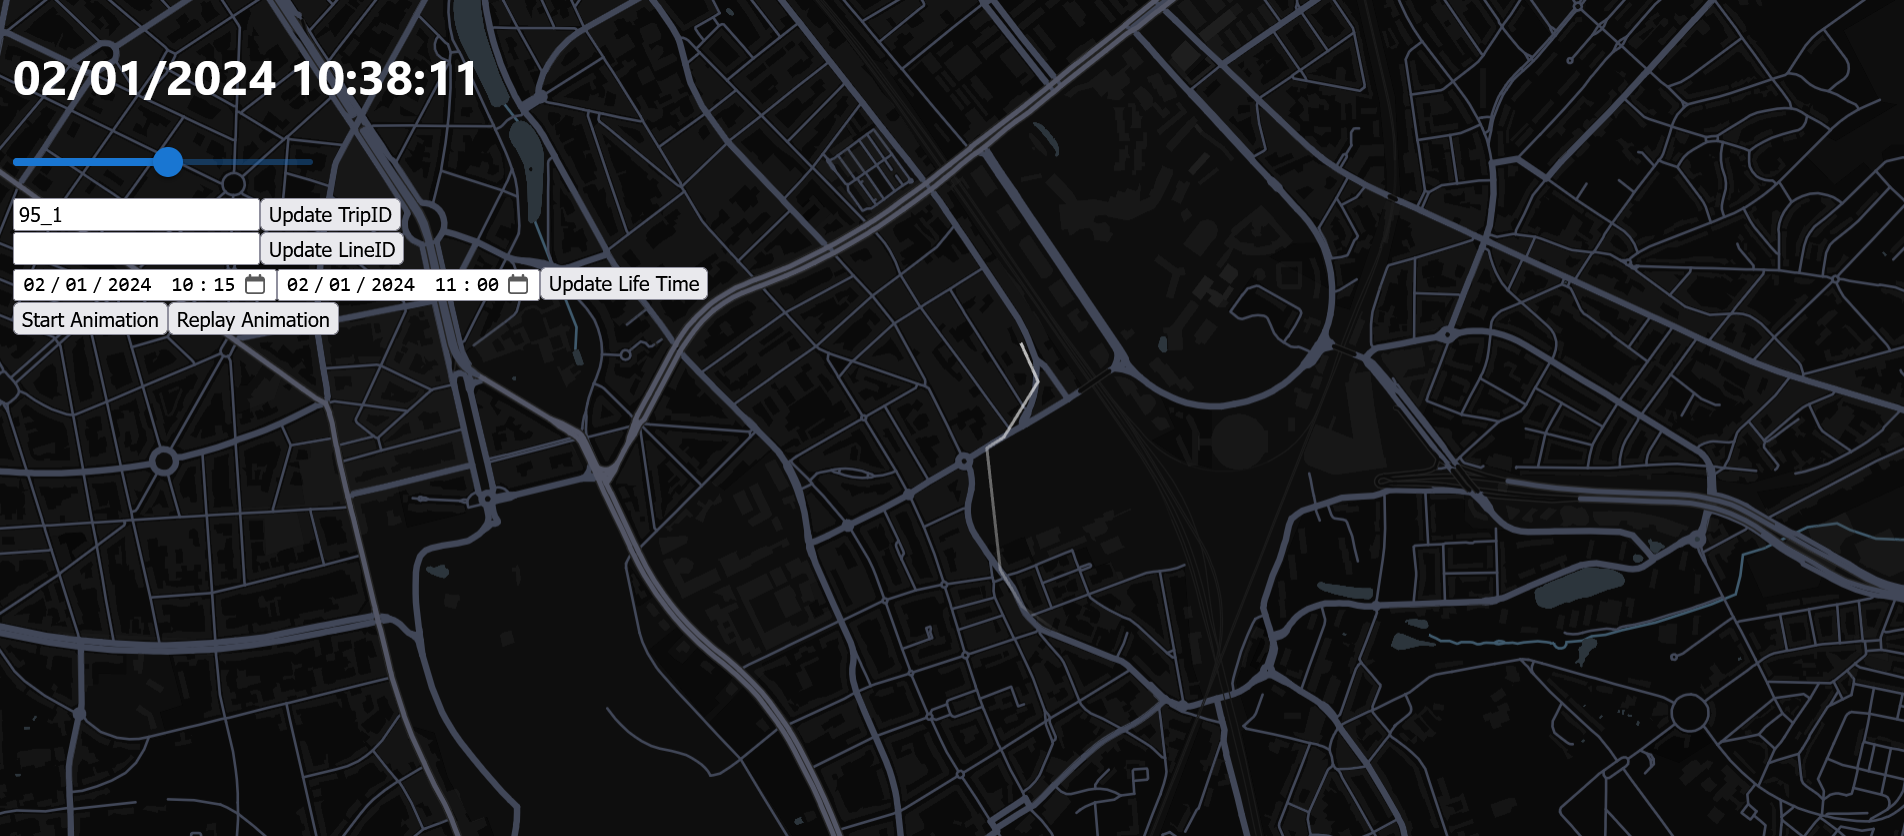
\includegraphics[width=0.9\textwidth]{images/GoodVisu.png}
			\caption{Displayed data make no sense}
			\label{GoodVisu}
		\end{figure}
	\end{center}
	
	When the underlying database retains data integrity, the module's visualization capabilities are excellent as  we can see in Figure \ref{GoodVisu}, highlighting its robust potential. Accurate data serves as the basis for the generation of consistent and precise visual narratives, enabling the module to vividly reconstruct the historical movements of vehicles on the network with remarkable fidelity. In cases where data is verified and reliable, visual outputs are not only accurate but also intuitive, facilitating an immersive analytical experience. Graphical renderings, in such cases, are seamless, providing a lucid and continuous representation of vehicle trajectories over time. This high-fidelity visualization is testament to the tool's sophisticated design and implementation, affirming its value as an essential asset for in-depth transit network analysis.
	
	As explained in the  previous section this result has been achieved by merging the power of multiples tools and the fact that pg\_tileserv can  handle requests for  multiple layers at the same time. For every layer tht we would  like to display on the screen there is an associated function layer written in postgresql and to which pg\_tileserv can acces and run to get the protibuf data that will be provided to the MVTLayer of DeckGL. Both function layers for the single vehicle visuliation and all the vehicles of the line are showed in \ref{lst:historicalTrip} and \ref{lst:historicalLine}. The forced conversion of the trips from SRID 4326 to SRID 3857 is due to the fact that pg\_tileserve default SRID is set to 3857 and proving data with different SRID make the resulting points to not be display at the right position because of the difference between every SRID has is own way to represent coordinates on a map. 
	
	
	\begin{lstlisting}[language=SQL,
		caption={Query to generate the protobuf data for one vehicle},
		label={lst:historicalTrip},
		basicstyle={\small\ttfamily},
		belowskip=3mm,
		breakatwhitespace=true,
		breaklines=true,
		classoffset=0,
		columns=flexible,
		commentstyle=\color{dkgreen},
		framexleftmargin=0.25em,
		frameshape={}{yy}{}{}, %To remove to vertical lines on left, set `frameshape={}{}{}{}`
		keywordstyle=\color{blue},
		numbers=left, %If you want line numbers, set `numbers=left`
		numberstyle=\tiny\color{gray},
		showstringspaces=false,
		stringstyle=\color{mauve},
		tabsize=3,
		xleftmargin =1em]
		CREATE OR REPLACE FUNCTION public.historical_trip(
		z integer, x integer, y  integer, p_tripid text, p_start text, p_end text)
		RETURNS bytea
		AS $$
		WITH bounds AS (
		SELECT ST_TileEnvelope(z,x,y) as geom
		),
		trips AS (
		SELECT asMVTGeom(transform(attime(trip,span(p_start::timestamptz, p_end::timestamptz, true, true)),3857),
		transform((bounds.geom)::stbox,3857)) as geom_times
		FROM stib_trips, bounds
		WHERE tripid = p_tripid
		),
		mvtgeom AS (
		SELECT (geom_times).geom, (geom_times).times
		FROM trips
		)
		SELECT ST_AsMVT(mvtgeom) 
		FROM mvtgeom
		$$
		LANGUAGE 'sql'
		STABLE
		PARALLEL SAFE;
	\end{lstlisting}
	
	\begin{lstlisting}[language=SQL,
		caption={Query to generate the protobuf data for all the vehicles of the  line},
		label={lst:historicalLine},
		basicstyle={\small\ttfamily},
		belowskip=3mm,
		breakatwhitespace=true,
		breaklines=true,
		classoffset=0,
		columns=flexible,
		commentstyle=\color{dkgreen},
		framexleftmargin=0.25em,
		frameshape={}{yy}{}{}, %To remove to vertical lines on left, set `frameshape={}{}{}{}`
		keywordstyle=\color{blue},
		numbers=left, %If you want line numbers, set `numbers=left`
		numberstyle=\tiny\color{gray},
		showstringspaces=false,
		stringstyle=\color{mauve},
		tabsize=3,
		xleftmargin =1em]
		CREATE OR REPLACE FUNCTION public.historical_line(
		z integer, x integer, y  integer, p_lineid text, p_start text, p_end text)
		RETURNS bytea
		AS $$
		WITH bounds AS (
		SELECT ST_TileEnvelope(z,x,y) as geom
		),
		trips AS (
		SELECT tripid,asMVTGeom(transform(attime(trip,span(p_start::timestamptz, p_end::timestamptz, true, true)),3857),
		transform((bounds.geom)::stbox,3857))
		as geom_times
		FROM stib_trips, bounds
		WHERE lineid = p_lineid
		),
		mvtgeom AS (
		SELECT (geom_times).geom, (geom_times).times,tripid
		FROM trips
		)
		SELECT ST_AsMVT(mvtgeom) 
		FROM mvtgeom
		$$
		LANGUAGE 'sql'
		STABLE
		PARALLEL SAFE;
	\end{lstlisting}
	
	
	
	
	
	\subsection{Real-Time visualization}
	The visualization module delineated in this section epitomizes a considerable stride in the real-time portrayal of geospatial transit data. Capitalizing on the sophisticated rendering capabilities of deck.gl and the efficiency of Mapbox Vector Tiles (MVT), this tool is pivotal in providing actionable insights into the Société des Transports Intercommunaux de Bruxelles (STIB) network operations. Through the graphic representation of vehicle positions—marked as nodes—on the network map, the system affords a detailed snapshot of the real-time movement of each vehicle, facilitating the discernment of transit patterns and vehicular flow.
	
	The provisioned Figure \ref{RTVisu}underscores the module's ability to trace individual vehicle trajectories, which are dynamically updated at intervals not exceeding 30 seconds. This frequent data refreshment ensures that stakeholders are equipped with the most current information, thereby supporting timely decision-making processes. Furthermore, the user interface is designed to enable focused examination of a single vehicle's route or, alternatively, an aggregated perspective of all vehicles on a selected line. Such a feature is instrumental for both immediate operational assessment and longitudinal data analysis, catering to varied analytical requirements.
	
	\begin{center}
		\begin{figure}
			\centering
			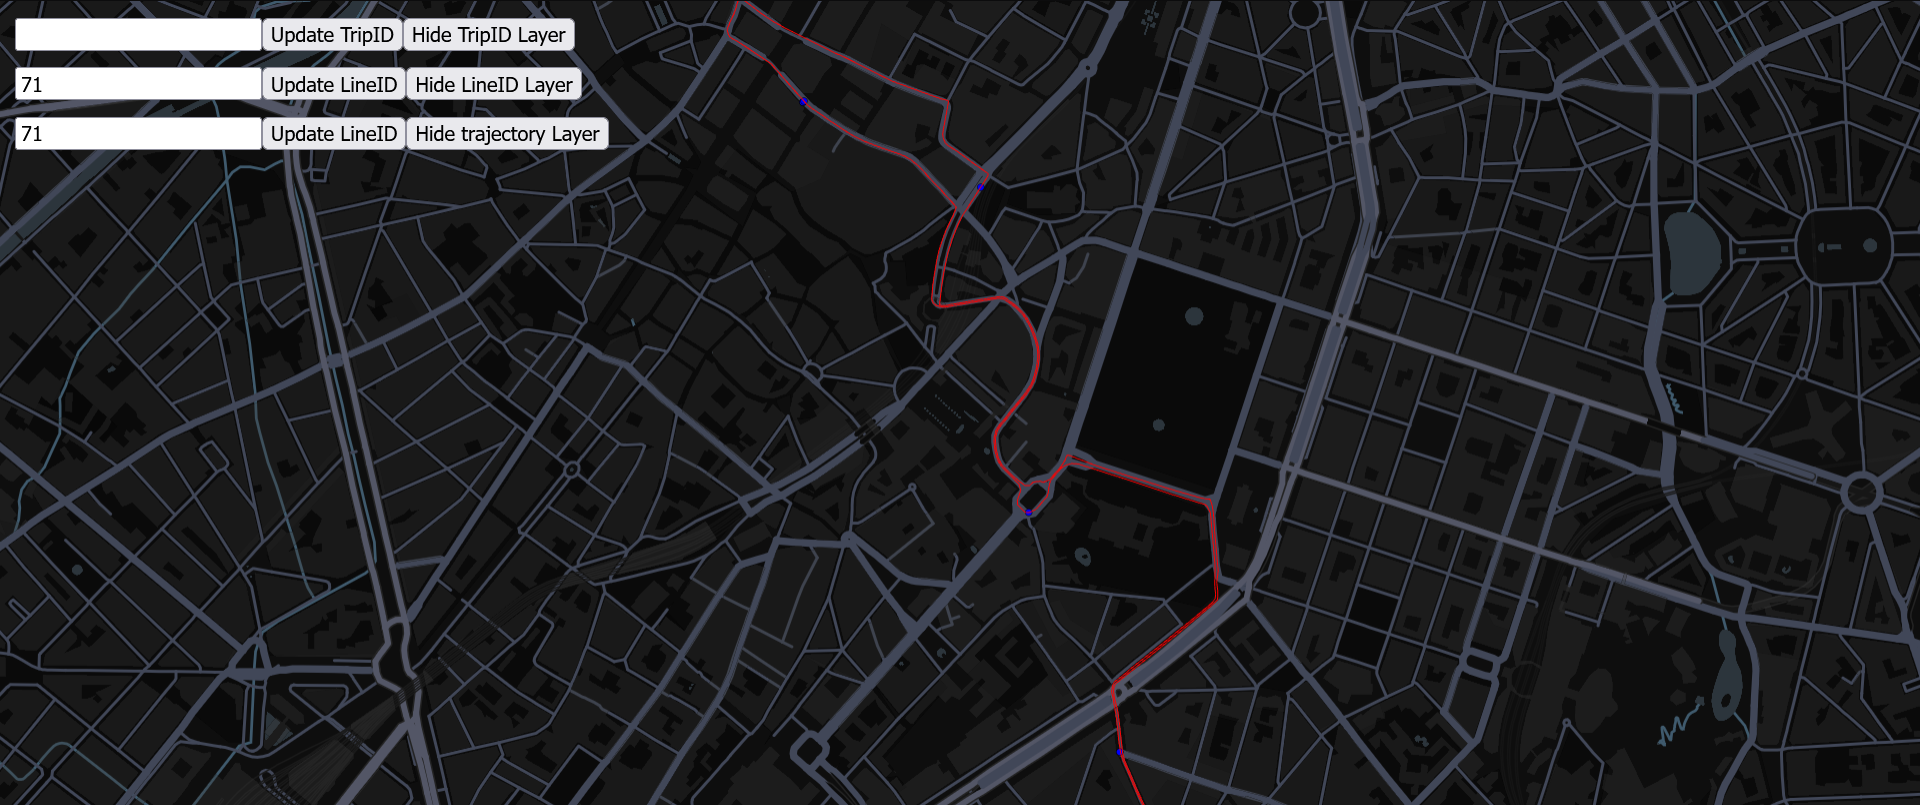
\includegraphics[width=0.9\textwidth]{images/RTVisu.png}
			\caption{Real-Time position of some vehicle of line 71}
			\label{RTVisu}
		\end{figure}
	\end{center}
	
	While deck.gl provides the robust data visualization infrastructure, the use of MVT facilitates the handling of extensive datasets with minimal performance impact, thus ensuring the tool's responsiveness and scalability. The interactive options presented, including 'Update TripID' and 'Hide TripID Layer', offer users a degree of customization in their interaction with the visualization, further extending its utility across multiple urban mobility research contexts.
	
	In conclusion, the visualization module presented here integrates advanced geospatial technologies to deliver a functional and responsive tool for urban transport visualization. It successfully furnishes a near-real-time overview of vehicle positions within the STIB network, albeit with the understanding that the fast-paced nature of urban transport may present challenges that this tool can only partially address. As such, while it stands as a valuable contribution to the field of urban mobility, the inherent limitations of real-time data analysis and the potential for information lag must be acknowledged. 
	
	As for the previous section in order to display the data on the screen a function layer has been written for every options that the users would display or not. The function are showed in \ref{lst:lastInstantTrip} for the function that allow to follow one vehicle in real-time, in \ref{lst:lastInstantLine} for the function that allow to follow all the vehicles of one line in real-time, and \ref{lst:trajectory} for the function that allow to display the entire trajectory that the vehicle is supposed to follow.
	
	\begin{lstlisting}[language=SQL,
		caption={Query to get the last position of the desired vehicle},
		label={lst:lastInstantTrip},
		basicstyle={\small\ttfamily},
		belowskip=3mm,
		breakatwhitespace=true,
		breaklines=true,
		classoffset=0,
		columns=flexible,
		commentstyle=\color{dkgreen},
		framexleftmargin=0.25em,
		frameshape={}{yy}{}{}, %To remove to vertical lines on left, set `frameshape={}{}{}{}`
		keywordstyle=\color{blue},
		numbers=left, %If you want line numbers, set `numbers=left`
		numberstyle=\tiny\color{gray},
		showstringspaces=false,
		stringstyle=\color{mauve},
		tabsize=3,
		xleftmargin =1em]
		CREATE OR REPLACE FUNCTION public.trip_last_instant(z integer, x integer, y integer, p_tripid text)
		RETURNS bytea
		AS $$
		WITH bounds AS (
		SELECT ST_TileEnvelope(z, x, y) AS geom
		),
		last_instant AS (
		SELECT tripid,asMVTGeom(transform(endinstant(trip), 3857), (bounds.geom)::stbox) AS geom_times
		FROM stib_trips, bounds
		WHERE tripid = p_tripid and current = true -- Filter by 'current' column
		),
		mvtgeom AS (
		SELECT (geom_times).geom, (geom_times).times
		FROM last_instant
		)
		SELECT ST_AsMVT(mvtgeom)
		FROM mvtgeom
		$$
		LANGUAGE 'sql'
		STABLE
		PARALLEL SAFE;
	\end{lstlisting}
	
	\begin{lstlisting}[language=SQL,
		caption={Query to get the last position of the vehicles of one line},
		label={lst:lastInstantLine},
		basicstyle={\small\ttfamily},
		belowskip=3mm,
		breakatwhitespace=true,
		breaklines=true,
		classoffset=0,
		columns=flexible,
		commentstyle=\color{dkgreen},
		framexleftmargin=0.25em,
		frameshape={}{yy}{}{}, %To remove to vertical lines on left, set `frameshape={}{}{}{}`
		keywordstyle=\color{blue},
		numbers=left, %If you want line numbers, set `numbers=left`
		numberstyle=\tiny\color{gray},
		showstringspaces=false,
		stringstyle=\color{mauve},
		tabsize=3,
		xleftmargin =1em]
		CREATE OR REPLACE FUNCTION public.line_last_instant(z integer, x integer, y integer, p_lineid text)
		RETURNS bytea
		AS $$
		WITH bounds AS (
		SELECT ST_TileEnvelope(z, x, y) AS geom
		),
		last_instant AS (
		SELECT asMVTGeom(transform(endinstant(trip), 3857), (bounds.geom)::stbox) AS geom_times
		FROM stib_trips, bounds
		WHERE lineid = p_lineid and current = true -- Filter by 'current' column
		),
		mvtgeom AS (
		SELECT (geom_times).geom, (geom_times).times
		FROM last_instant
		)
		SELECT ST_AsMVT(mvtgeom)
		FROM mvtgeom
		$$
		LANGUAGE 'sql'
		STABLE
		PARALLEL SAFE;
	\end{lstlisting}
	
	\begin{lstlisting}[language=SQL,
		caption={Query to the trajectory of the desired line},
		label={lst:trajectory},
		basicstyle={\small\ttfamily},
		belowskip=3mm,
		breakatwhitespace=true,
		breaklines=true,
		classoffset=0,
		columns=flexible,
		commentstyle=\color{dkgreen},
		framexleftmargin=0.25em,
		frameshape={}{yy}{}{}, %To remove to vertical lines on left, set `frameshape={}{}{}{}`
		keywordstyle=\color{blue},
		numbers=left, %If you want line numbers, set `numbers=left`
		numberstyle=\tiny\color{gray},
		showstringspaces=false,
		stringstyle=\color{mauve},
		tabsize=3,
		xleftmargin =1em]
	\end{lstlisting}
	
	
	\section{\acrshort{stib} Alarms}
	
	In this section we will discuss about the alarm system that has been created in order to help BM detect vehicles that are likely blocked on their path and that can create a lot of troubles in the traffic fluidity which is the most important thing for BM and why it is unfortunately for the moment not enough precise to consider all the alarms as correct.
	
	The catalog of error messages communicated to Brussels Mobility (BM) plays a pivotal role in the optimization of traffic flow. To achieve the intended outcome, we have employed the stops function from MobilityDB. The query used in order to achieve the  result is \ref{lst:stopsQuery}. 
	
	\begin{lstlisting}[language=SQL,
		caption={Query to generate the  alarm for every vehicle that is currently onthe network},
		label={lst:stopsQuery},
		basicstyle={\small\ttfamily},
		belowskip=3mm,
		breakatwhitespace=true,
		breaklines=true,
		classoffset=0,
		columns=flexible,
		commentstyle=\color{dkgreen},
		framexleftmargin=0.25em,
		frameshape={}{yy}{}{}, %To remove to vertical lines on left, set `frameshape={}{}{}{}`
		keywordstyle=\color{blue},
		numbers=left, %If you want line numbers, set `numbers=left`
		numberstyle=\tiny\color{gray},
		showstringspaces=false,
		stringstyle=\color{mauve},
		tabsize=3,
		xleftmargin =1em]
		select  lineid,trip_headsign,astext(unnest(sequences(stops(trip,5,'5 minutes'))))
		from stib_trips as st, terminus_shapes as ts
		where tempSubType(trip) !=  'Instant' and  current = true and  ts.route_short_name  = st.lineid
		group by trip,lineid,trip_headsign;
	\end{lstlisting}
	
	
	
	This function is instrumental in analyzing MobilityDB trip data to pinpoint instances where a vehicle remains within a confined spatial radius—defined by a predetermined size—for a minimum duration threshold. In this context, our parameters were set to identify vehicular stagnation exceeding a 5-meter radius for a duration of no less than 5 minutes. Upon detection of such an event, our system triggers an alarm that is subsequently encoded into a JSON file. This file is then dispatched to the relevant operational personnel for further examination and intervention as deemed necessary. This procedure is integral to the proactive management of traffic and the mitigation of potential congestion.
	
	The output of the file is given by the image \ref{img:AlarmSTIB}, we can see that for every alarm there is multiples fields that can help the operator to understand where and since when the problem is occurring.
	
	\begin{center}
		\begin{figure}
			\centering
			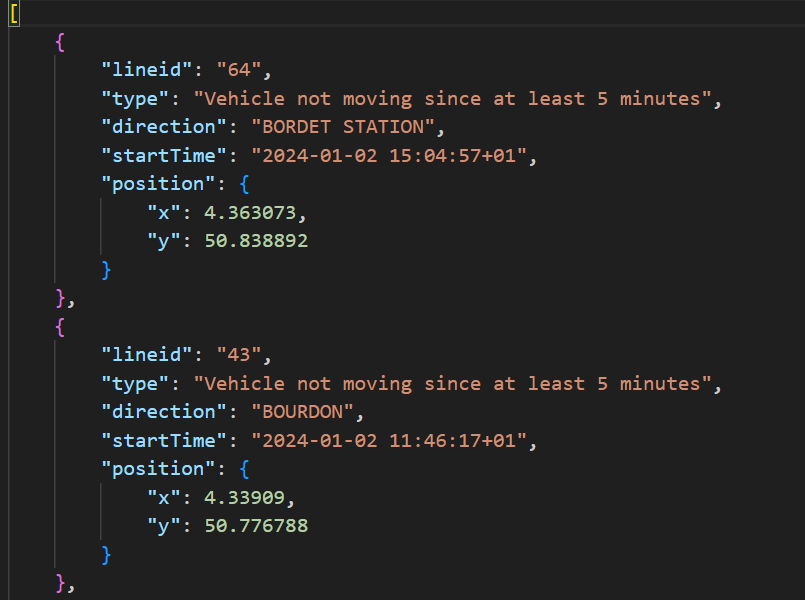
\includegraphics[width=0.9\textwidth]{images/alarmSTIB.png}
			\caption{Example of alarm file}
			\label{alarmSTIB}
		\end{figure}
	\end{center}
	
	Because of the problems mentioned in the previous Sections all the alarms are not 100\% reliable, but as soon as all the vehicles of the STIB will have an unique identifier for every vehicles all the features already implemented will be 100\% functional. 
	
	
	
	\chapter{Future work}
	
	This study has allowed MobilityDB to start investing the path to be one of the main tool to handle the traffic in the city of Brussels. Nevertheless there is still a lot of possibilities to explorer that can lead to the implementation of new functionalities in MobilityDB that would make this extension even more efficient.
	
	\section{\acrshort{stib} Trips}
	
	The feature presented here represents the crux of this study and will be instrumental in shaping future work. Discussions are underway between BM and STIB to ascertain a timeline for the enhancement of STIB's real-time positioning system, with improvements projected to be completed by 2025. To refine the current system, it is necessary to devise an intricate algorithm that preserves each incoming data batch for comparison with its predecessor. This process will involve numerous interactions with the database to accurately identify consistent vehicle trajectories between successive batches.The challenge lies in the brief 20-second intervals between batch arrivals, which complicates the task of processing the entirety of the network's vehicular data. Currently, the system manages to update all trip details within an average span of 4 seconds during midday peaks. Incorporating these extensive computations is likely to extend processing times beyond the 20-second mark, potentially leading to data omission. Furthermore, while this proposed solution aims to minimize data inaccuracies, it acknowledges the inevitability of residual errors within the datasets.
	
	
	\section{\acrshort{stib} Alarms}
	
	The STIB alarm system is slated for an upgrade to align with the expected improvements to STIB's real-time positioning system by 2025. This enhancement is crucial for efficiently identifying and addressing service disruptions that could impact traffic flow and service reliability.
	
	In case we would augment the current system alarm before 2025 a focus will be placed on refining the method of trip construction. This will involve the implementation of an improved approach to process and analyze incoming data more accurately. The aim is to enhance the alarm system's ability to track vehicles and detect anomalies more precisely, thereby reducing false positives and increasing overall system reliability.
	
	A key challenge in this upgrade is to manage the increased data processing requirements within the limited time frame available between data batches. The current system updates trip information in about 4 seconds during peak times, and it is vital to ensure that the enhanced system does not exceed this update interval. Efficient processing is essential to prevent data loss and maintain the system's effectiveness.
	
	This upgrade of the STIB alarm system is a critical aspect of our future work. It represents an opportunity to showcase the capabilities of MobilityDB and its application in a real-world, high-impact scenario. The successful refinement of this system will be a significant step forward in advancing urban traffic management solutions.
	
	
	\section{Vehicle Counting (M3)}
	\label{sec:futurWorkM3}
	
	The work of associating M3 count data with MobilityDB is independent of what was presented in the previous sections. There are still many possibilities to be explored, but a first avenue to explore would be to use MobilityDB's tint type to create a history of count data that would firstly be stored in a more efficient way by removing all the superfluous data we saw in Section \ref{sec:dataM3}, but which would also allow visualization over time just as has been done with vehicle trip data from the STIB network. For the visualization, we could imagine a circle that increases or decreases in size around the point where the camera is located over time, to show the density of vehicles around the camera.
	
	\section{Traffic Lights States (TLC)}
	\label{sec:futurWorkTLC}
	
	As with the data in the previous section, no real results could be obtained from the data provided by TLC. However, it would be very interesting to be able to look into this, knowing that red light data can provide a great deal of insight into the traffic situation at any given moment, and that being able to manage red light behavior in a city can greatly improve traffic flow at critical points during rush hour, or even help understand what happened at a point where there was a problem with traffic flow. 
	
	\section{Visualization Tool}
	
	As explained in the previous sections this implementation depends from the implementation of the STIB trips and the analyses of  other data sources to which BM could have the access to. Nevertheless we can imagine  additional features depending on the user requirements. The possibilities of information that we can display from the static GTFS data and the constructed  MobilityDB trips are numerous
	but a good  knowledge of the problems that are related to traffic flow  is necessary in order to develop the right visualization.
	
	We can imagine an improvement of the tool as being the addition of the visualization of counted vehicles around an area and  the state of the traffic lights and then replay the situation and analyze from where was the problem coming, was it a vehicle blocking the road or to  much vehicles in the area by looking at the counting or the traffic light behavior that wasn't adapted to the flow at that moment and a lot  of other scenarios like that. 
	
	\chapter{Conclusion}
	
	This study has illuminated the transformative capabilities of MobilityDB for enhancing urban traffic management in Brussels. Through the integration and analysis of real-time and historical data from STIB's network, we have established a foundational framework that sets the stage for a transport system that is both intelligent and adaptable.
	
	The implementation of the features discussed herein not only serves immediate operational needs but also opens a myriad of possibilities for MobilityDB. This project has presented an invaluable opportunity to demonstrate the full potential of this extension. Its success lays testament to the versatility and strength of MobilityDB in handling complex spatiotemporal data.
	
	The current phase of our research has been primarily devoted to solidifying reliable data streams and crafting initial analytical tools. However, the journey ahead is filled with potential. The forthcoming enhancements to STIB's real-time positioning system, expected to be complete by 2025, will play a critical role. Moreover, the sophisticated algorithm planned for implementation aims to further refine the accuracy of data processing. It is important to bear in mind, nonetheless, that some level of imperfection is inherent in real-time data analytics.
	
	In sum, the advancements made thus far are significant and indicative of a positive trajectory. Yet, the pursuit of a fully optimized, data-driven transit system for Brussels remains a work in progress. The sustained pursuit of innovation, together with upcoming improvements in STIB's data infrastructure, will undoubtedly enable more efficient and dependable urban transportation solutions. Through these efforts, MobilityDB stands to not only prove its worth but also to carve a niche as an indispensable tool in the realm of geographic information systems.
	
	
	
	\printbibliography	
\end{document}